\section{Experiments and Results} \label{sec:result}

\changed{ \subsection{Experimental Design}
We first validate the proposed algorithms on the fruit and city
datasets~\cite{zeiler2010deconvolutional}, where each consists of 10
training images of size $100 \times 100$. The online-mode algorithms
are then adapted to one thousand $100 \times 100$ image patches
randomly picked up from ImageNet~\cite{deng2009imagenet}. Note that batch-based CSC commonly can only handle less than 100 images
simultaneously due to the memory limitation. The dictionary size is set to $100$ filters of size $11 \times 11$ pixels in all experiments except for over-complete dictionary. All training and evaluation processes in this manuscript are performed on contrast normalized
images~\cite{zeiler2010deconvolutional,heide2015fast}.}

\begin{figure}[h]
\centering
\begin{subfigure}{0.45\textwidth}
  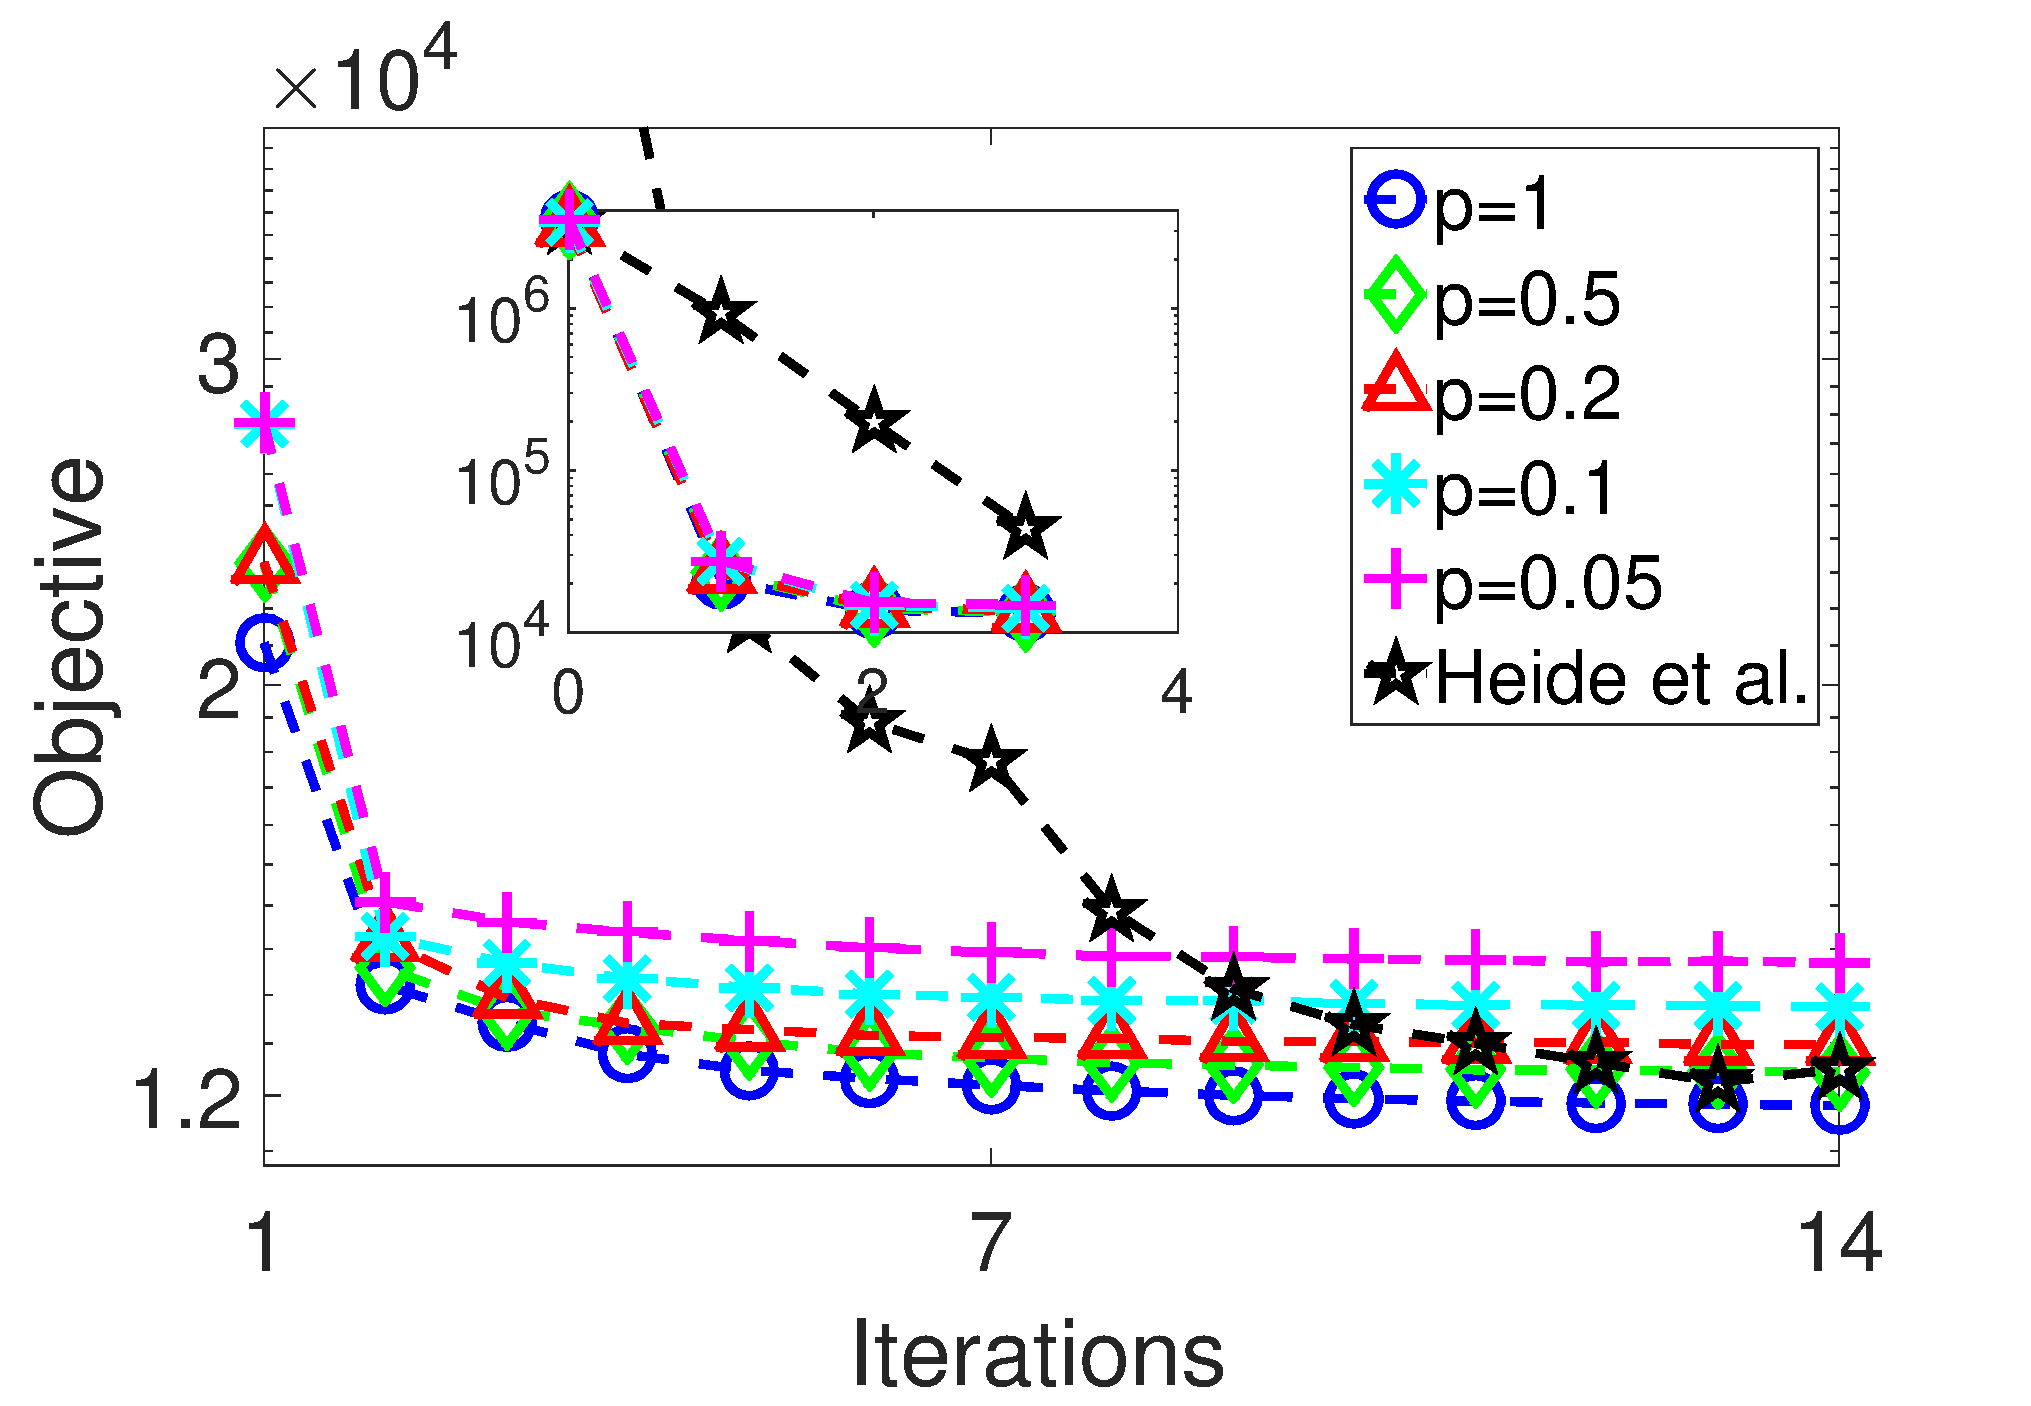
\includegraphics[width=1\linewidth]{figure/iteVSobj.pdf}
\end{subfigure}

\begin{subfigure}{0.45\textwidth}
  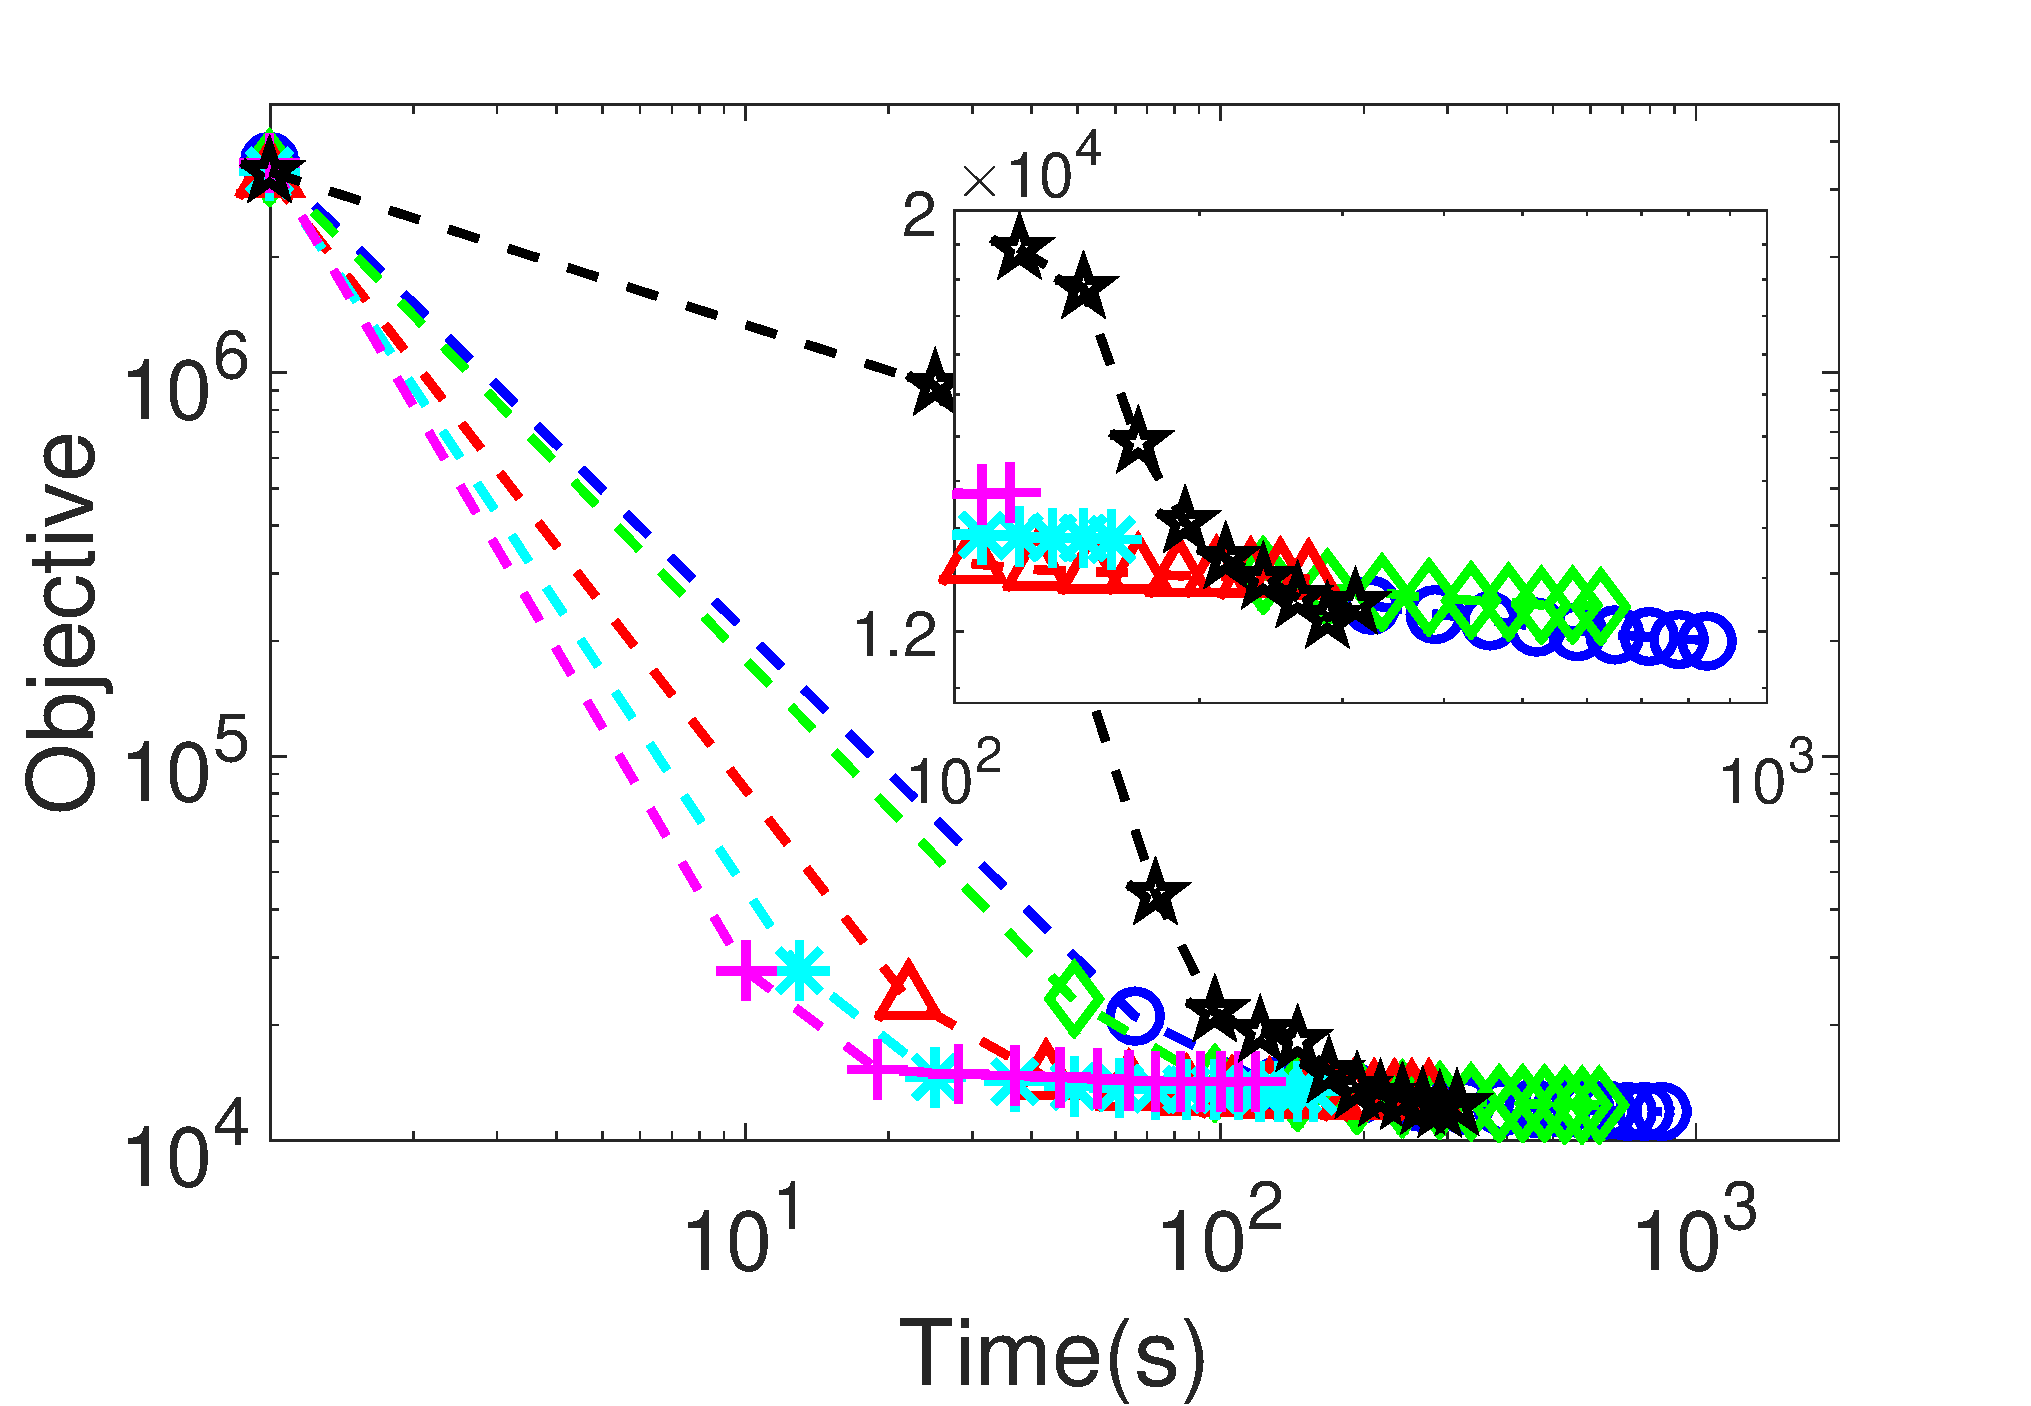
\includegraphics[width=1\linewidth]{figure/timeVSobj.pdf}
  \vspace*{1mm}
\end{subfigure}

%\begin{subfigure}{0.23\textwidth}
%  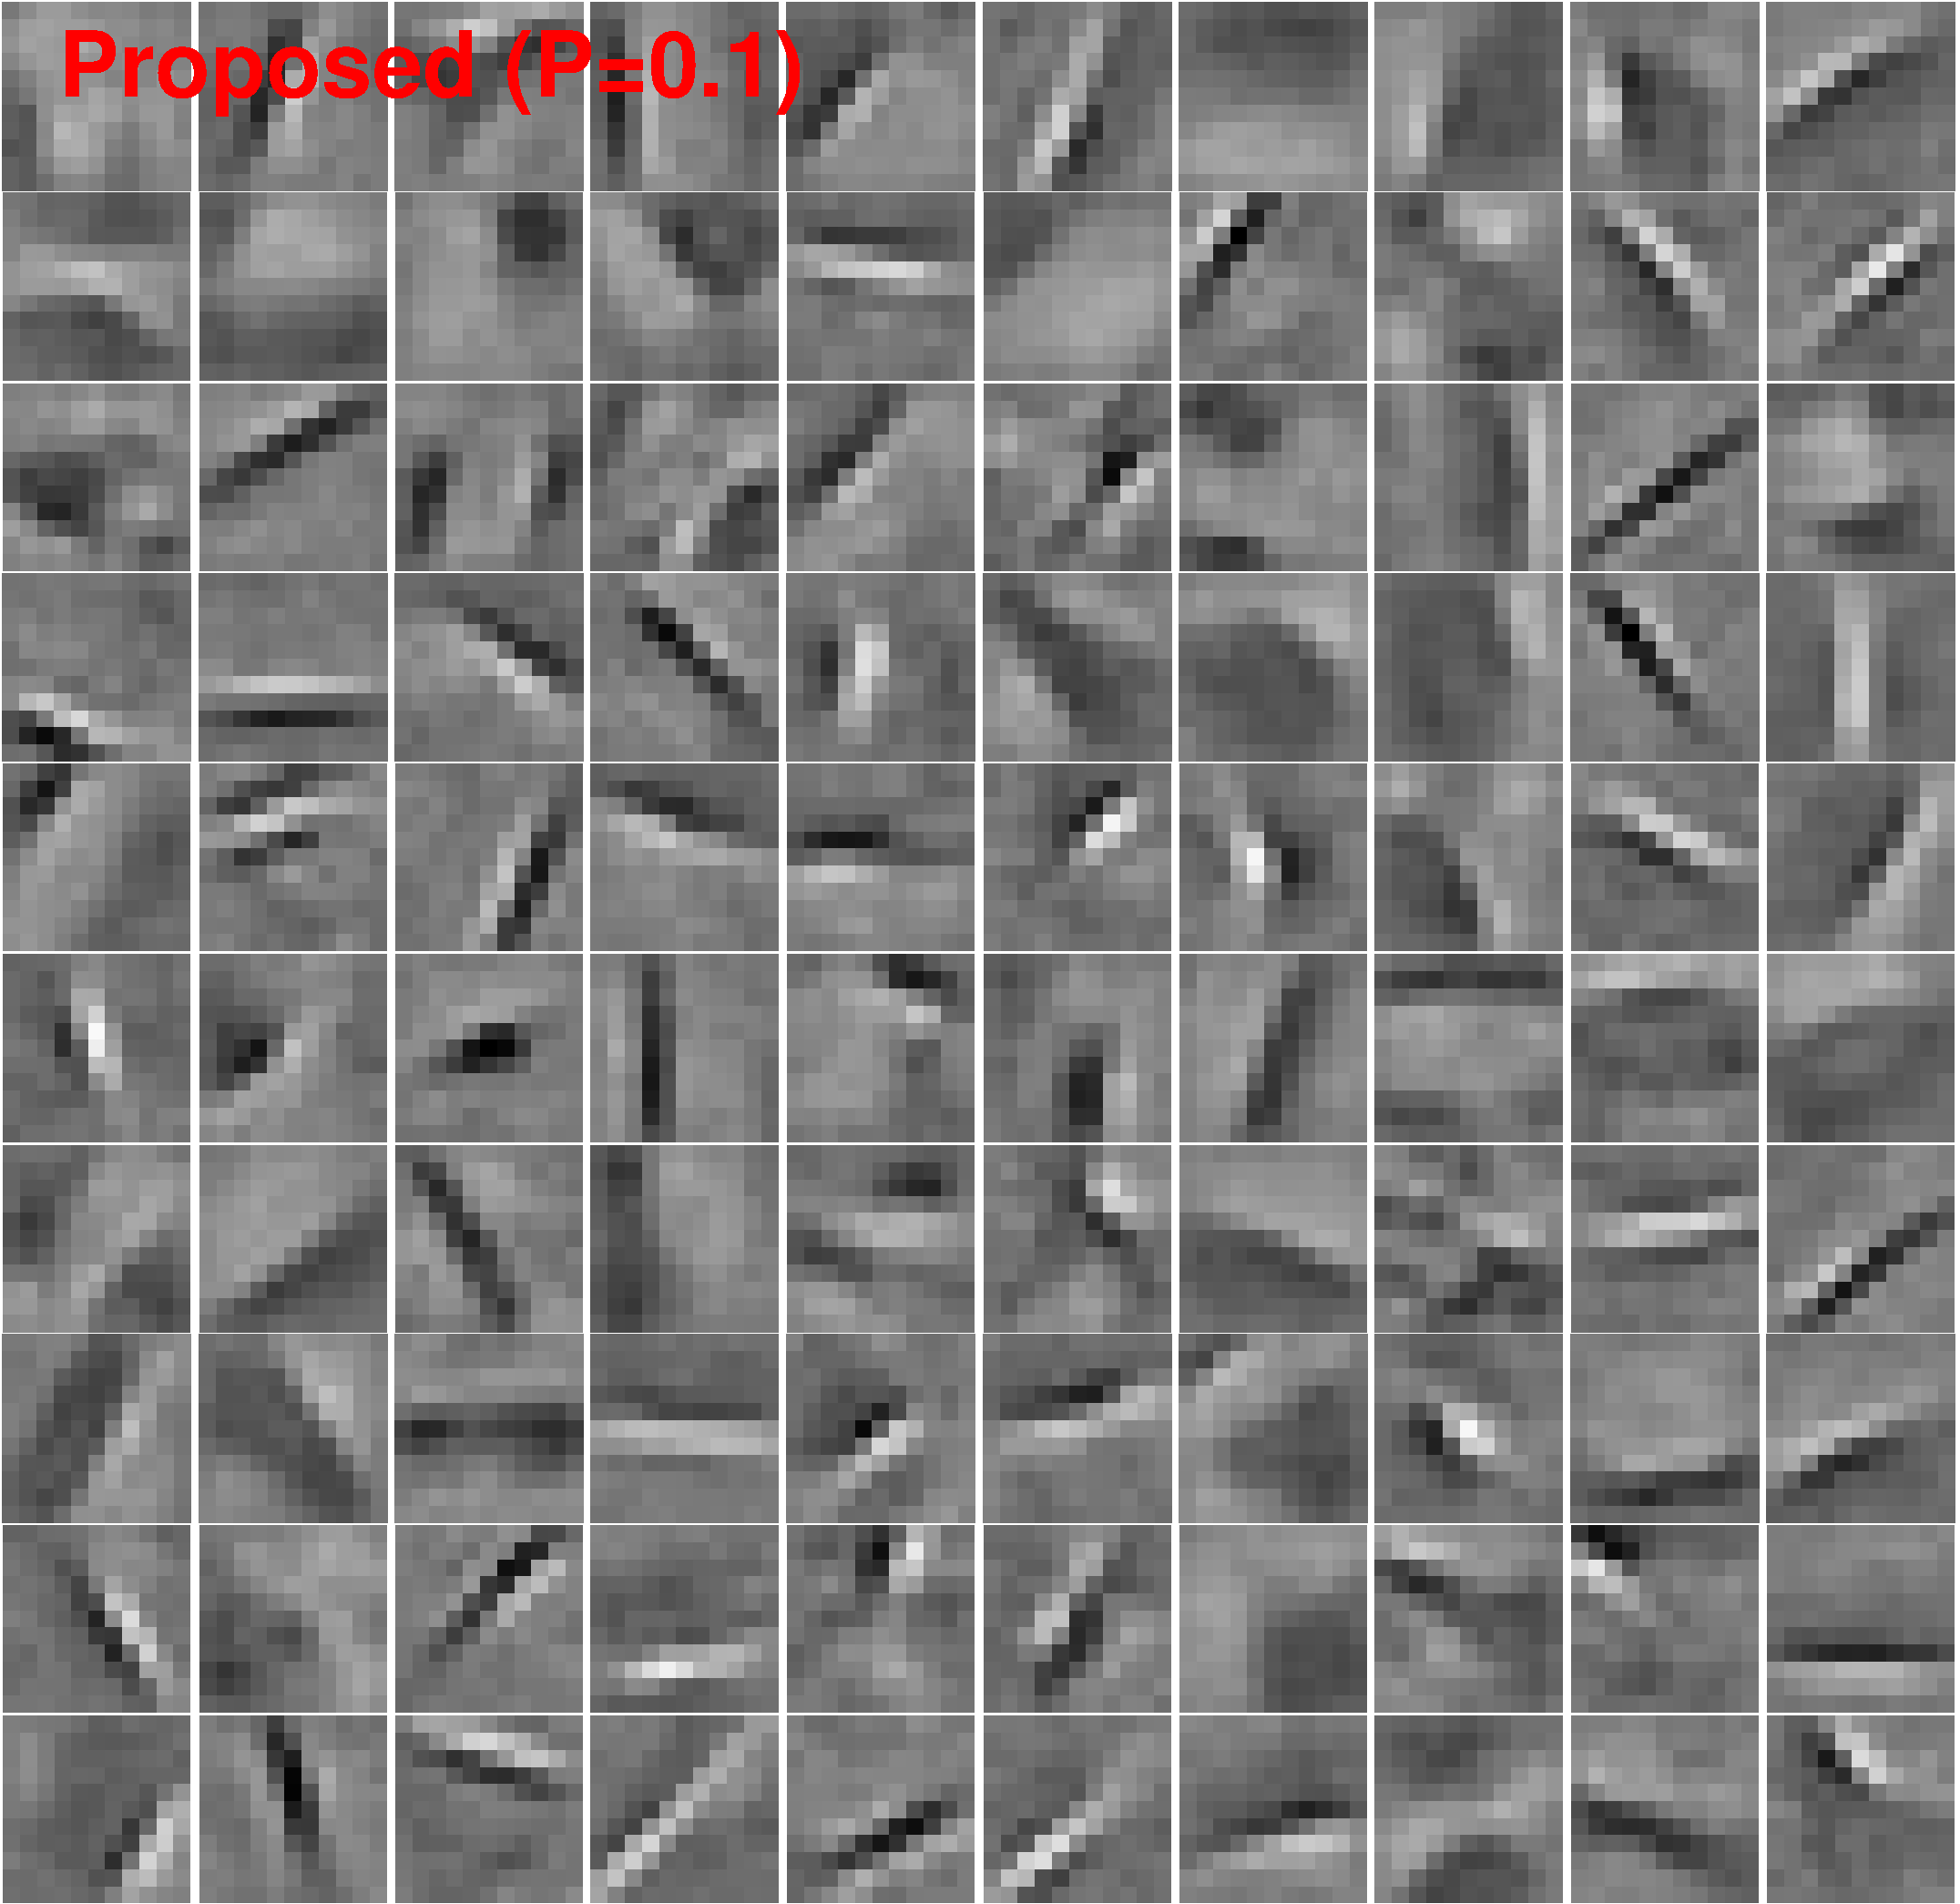
\includegraphics[width=1\linewidth]{figure/batchFruit100.pdf}
%\end{subfigure}
%\begin{subfigure}{0.23\textwidth}
%  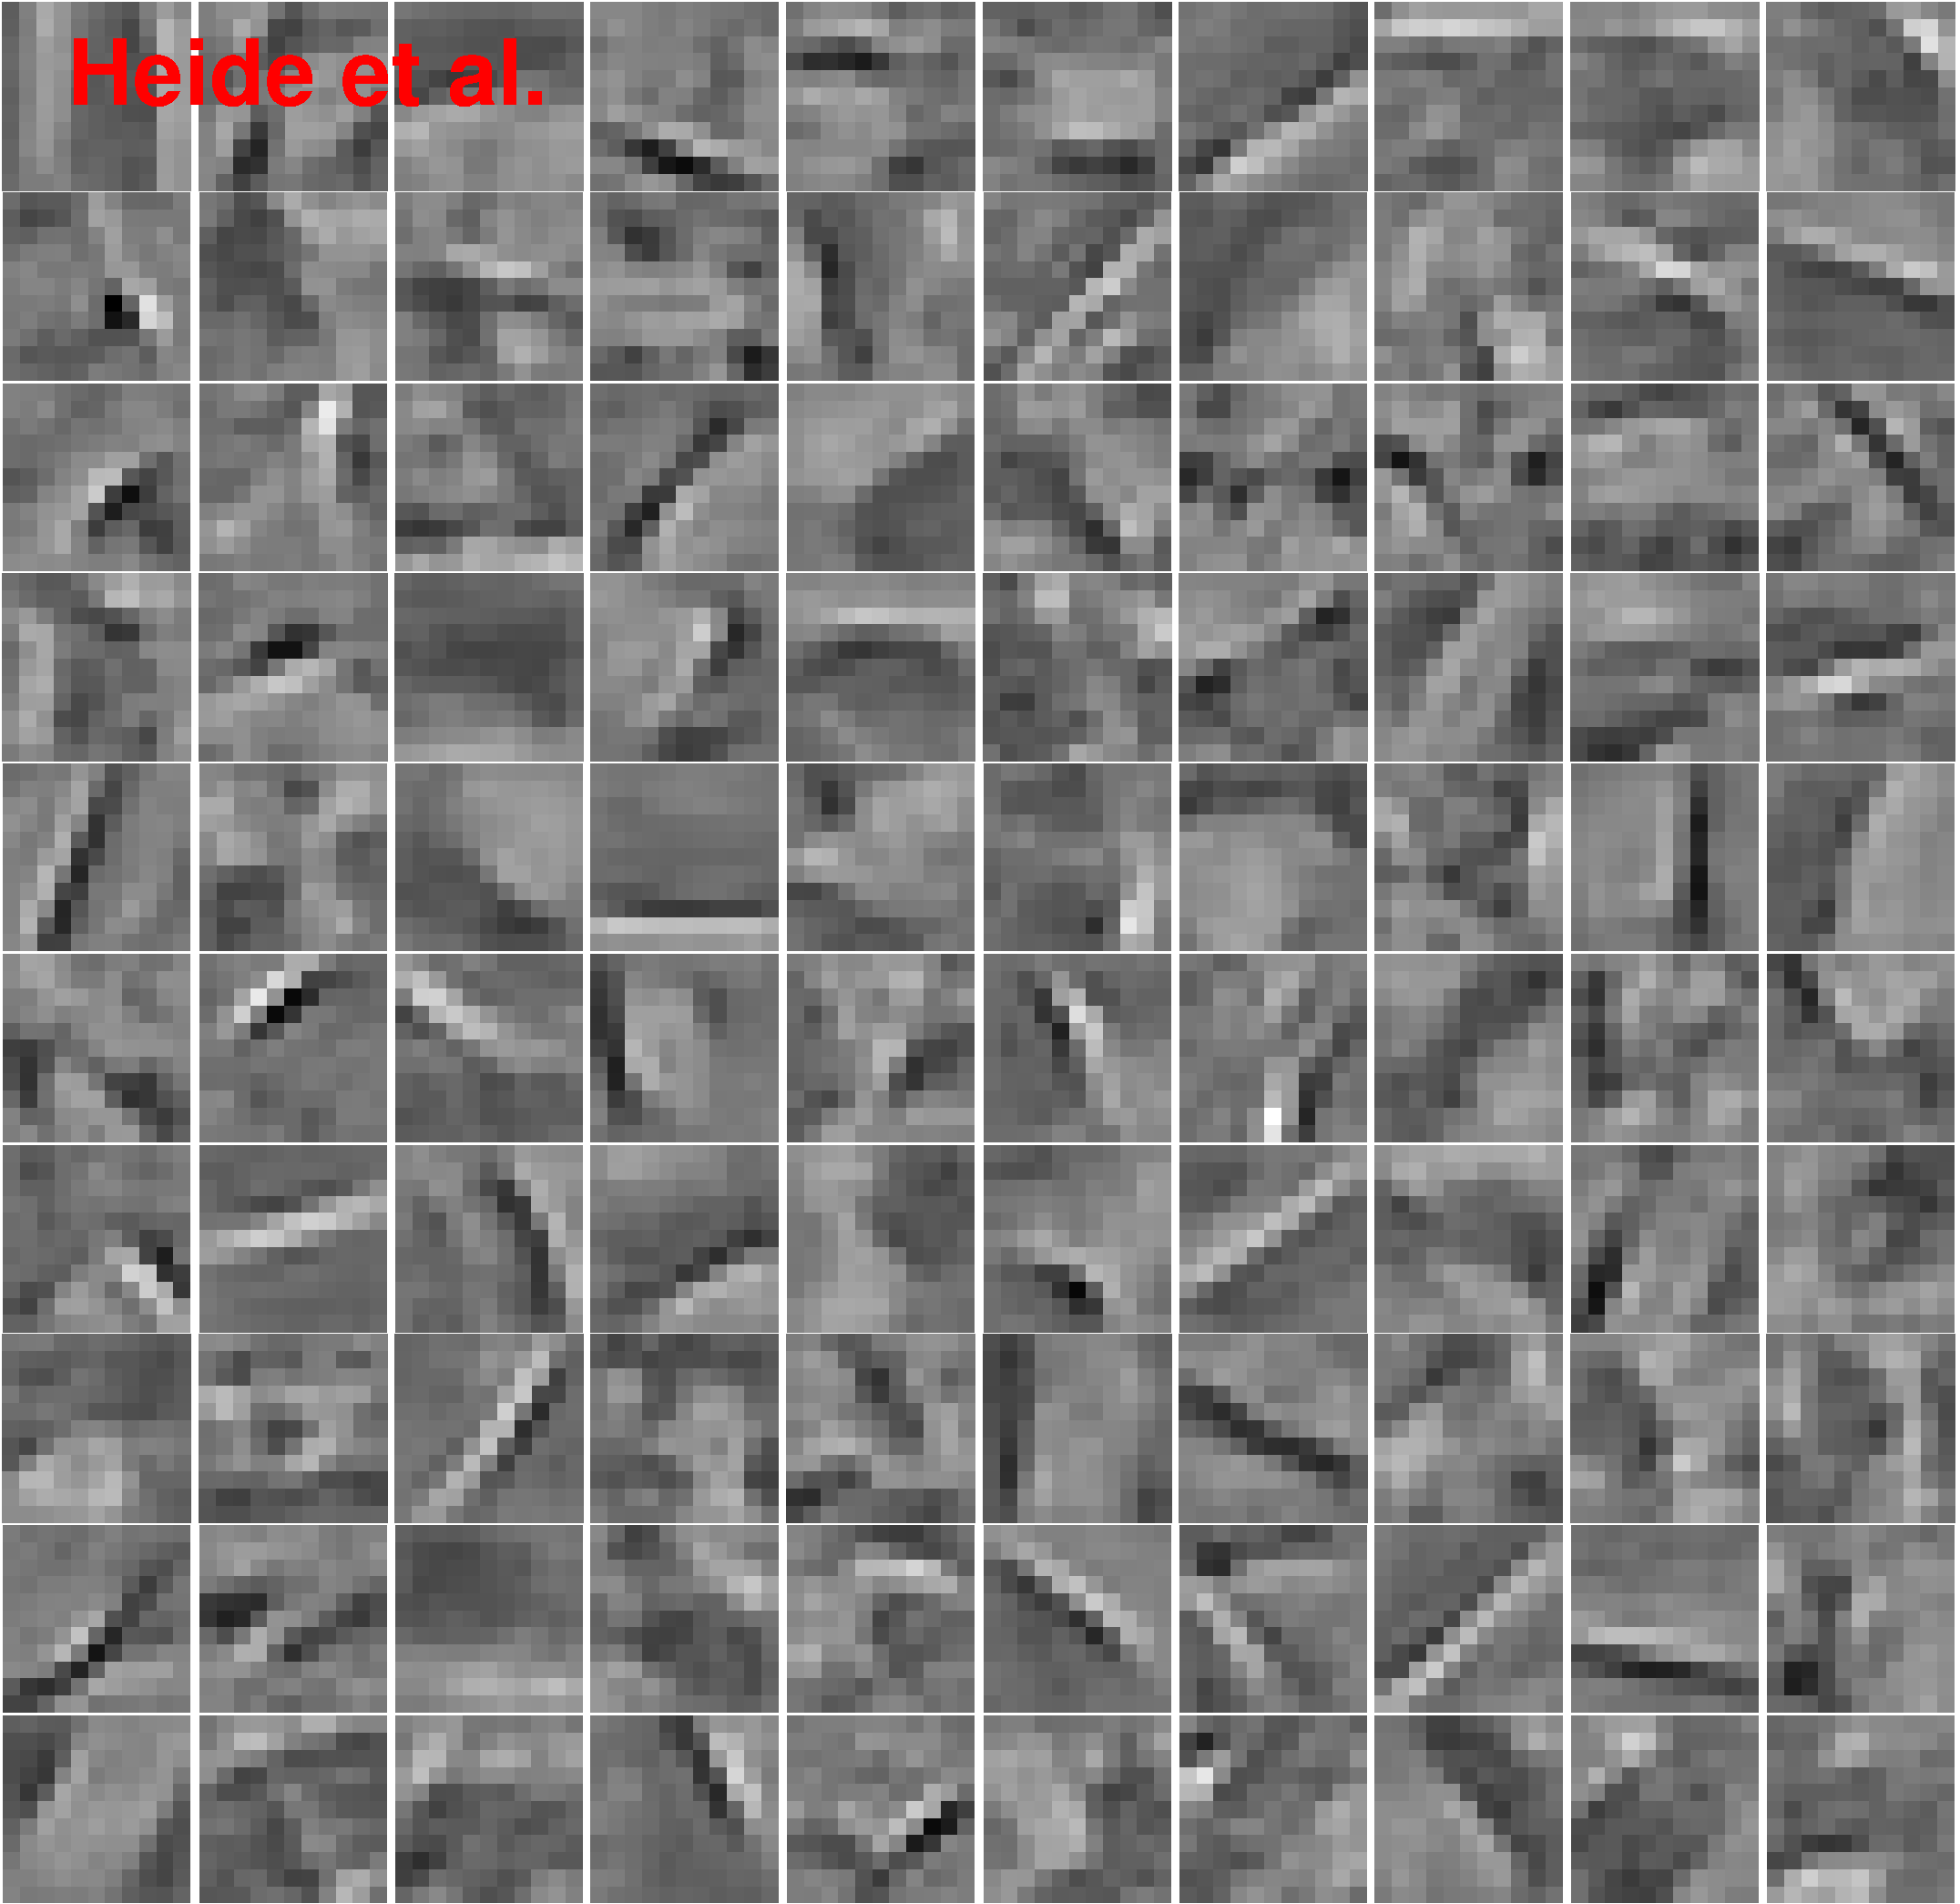
\includegraphics[width=1\linewidth]{figure/heideFruit100.pdf}
%\end{subfigure}
\caption{Convergence comparison between the-state-of-art method~\cite{heide2015fast} and the proposed method with different subsampling rate, all of which are performed on fruit dataset. Convergence is evaluated by monitoring the objective value of Eq.~\ref{eq:CSCmodel} on training images versus iterations and time, respectively.}
\label{fig:subsampleResult}
\end{figure}

\subsection{Subsampling Strategy}

{\bfseries Convergence.} Comparisons of the convergence between the
proposed method (SBCSC) and the state-of-the-art batch-mode
algorithm~\cite{heide2015fast} are shown in
Fig.~\ref{fig:subsampleResult} \changed{(the compared method uses a similar number of iterations as ours to reach convergence)}. A different selection of the
subsampling rate reveals that the proposed strategy will slightly
influence the convergence and the training objective of the
minimization problem. Specifically, the more subsampled, the
relatively slower convergence and the higher objective will be
obtained. On the other hand, small subsampling rate will significantly
accelerate the computation process, where $10\%$ subsampling achieves
about $6 \times$ speedup over the not subsampled spatial domain solver
and a $2 \times$ speedup over state-of-the-art Frequency-domain solver
for one iteration. We observe that a subsampling rate between $p=0.1$
and $p=0.2$ delivers empirically good enough convergence in our
settings, as well as achieving at least $3 \times$ speedup. In
general, the proposed method with various subsampling rates converges
at around 10-12 iterations in all testing cases, acting similar to the
competing methods.

%We have observed that the comparison method has a relatively
%high objective value during the first $6-8$ iterations. The reason is that it introduces an additional mask term handling the boundary issues, therefore different splitting strategies are utilized and the subproblems are
%interleaved on their primary variables (in some sense, the primary variables can be regarded as intermediate results in the ADMM iteration). See~\cite{wohlberg2016efficient} for details. Despite of this, it converges to an optimum with comparable objective after 10 iterations.
In summary, the convergence behaviors of the proposed
algorithm is only slightly influenced by the subsampling strategy
within the testing subsampling rates. Comparing to the
state-of-the-art frequency solver, the proposed stochastic
spatial-domain solver with a subsampling rate of $0.1$ reduces the
computation time by a factor of two for the tested example. Specifically,
SBCSC takes 170 seconds and the comparable method takes 350 seconds for
14 iterations on a Core i7 PC. The
robustness of the proposed algorithm is evaluated by additional
experiments. Please see supplementary materials for reference.

%{\bfseries Reconstruction}. The SBCSC-learned filters with a
%subsampling rate of $p=0.1$ are shown in the bottom of
%Fig.~\ref{fig:subsampleResult}. For a visual comparison, we also show
%the filters learned from the competing method (bottom left of Figure 3
%in~\cite{heide2015fast}). As can be observed, both of them learn some
%seemingly similar Gabor-like filters. However, zooming into the
%details (please see supplemental materials for high resolution
%versions) reveals that our filters appear less noisy than the ones
%from~\cite{heide2015fast}. We then demonstrate the effectiveness of
%the reconstructed filters in the application of image inpainting,
%which refers to reconstructing a full image from partial
%measurements. A numerical comparison of the reconstruction quality is
%shown in Fig.~\ref{fig:PSNRrecon}. The filters learned by the proposed
%method not only appear less noisy by themselves, but also achieve
%better reconstruction quality on partially observed images with
%respect to the PSNR value. Furthermore, the learning process
%only takes about $50\%$ of the time for our method. Specifically, SBCSC takes 170 seconds and the comparable method takes 350 seconds for 14 iterations on a Core i7 PC.

\subsection{Online Learning}

\begin{figure}[h]
\centering
\begin{subfigure}{0.45\textwidth}
  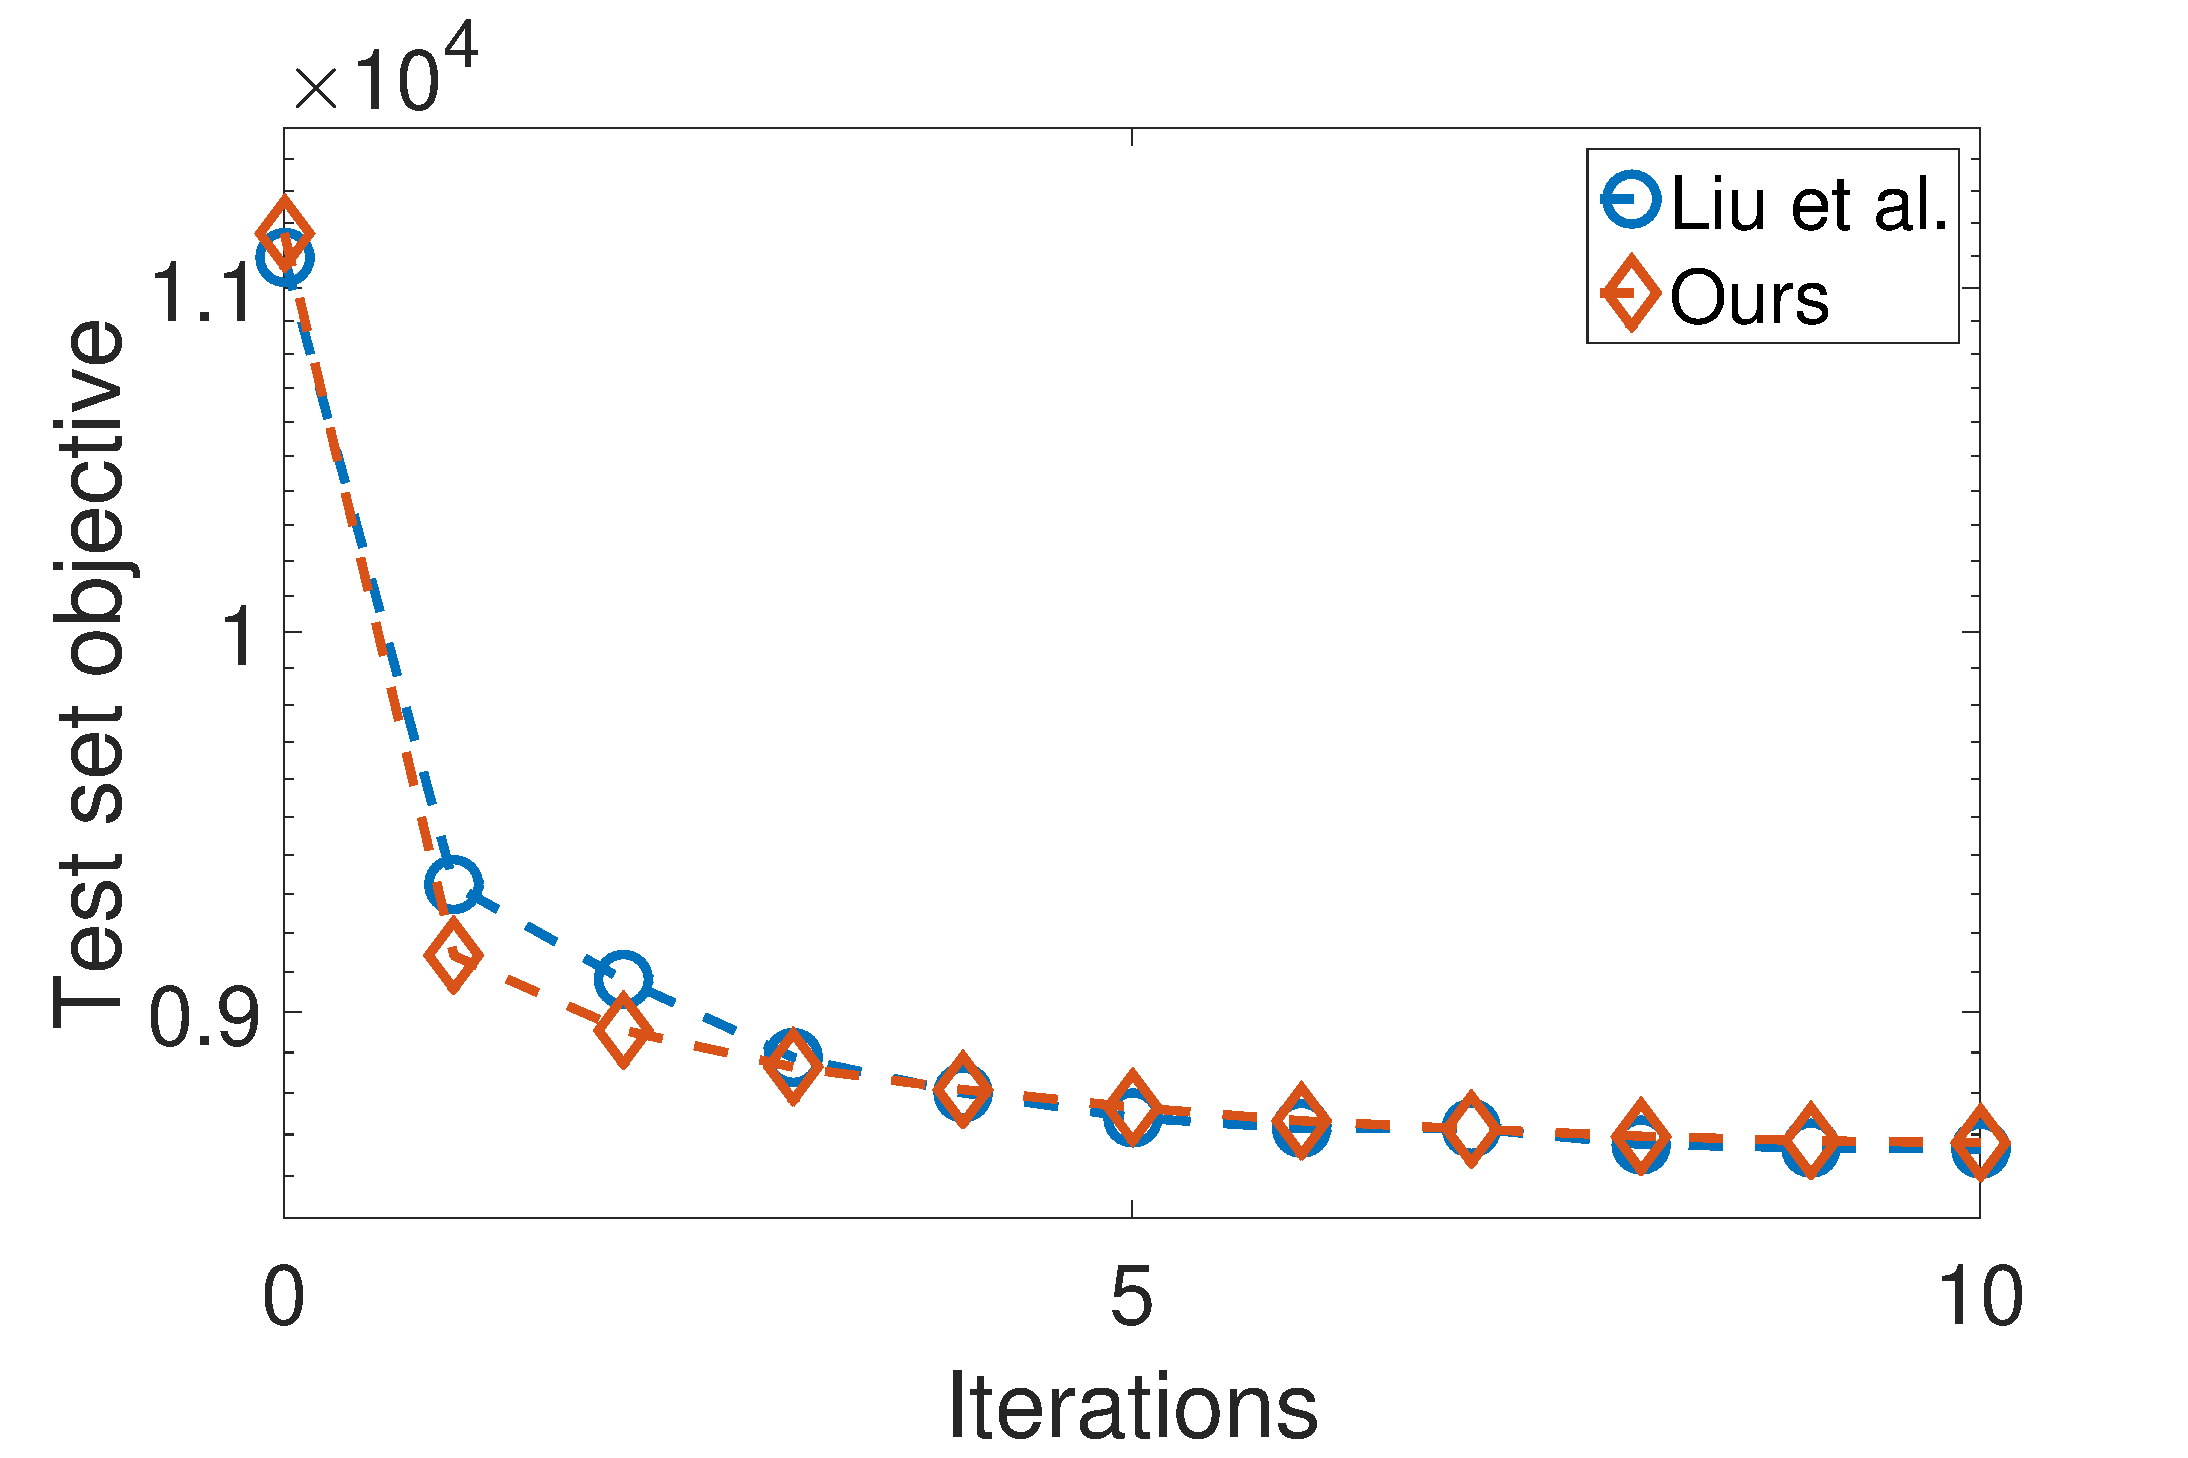
\includegraphics[width=1\linewidth]{figure/onlineVSliu-ite-fruit.pdf}
\end{subfigure}
\begin{subfigure}{0.45\textwidth}
  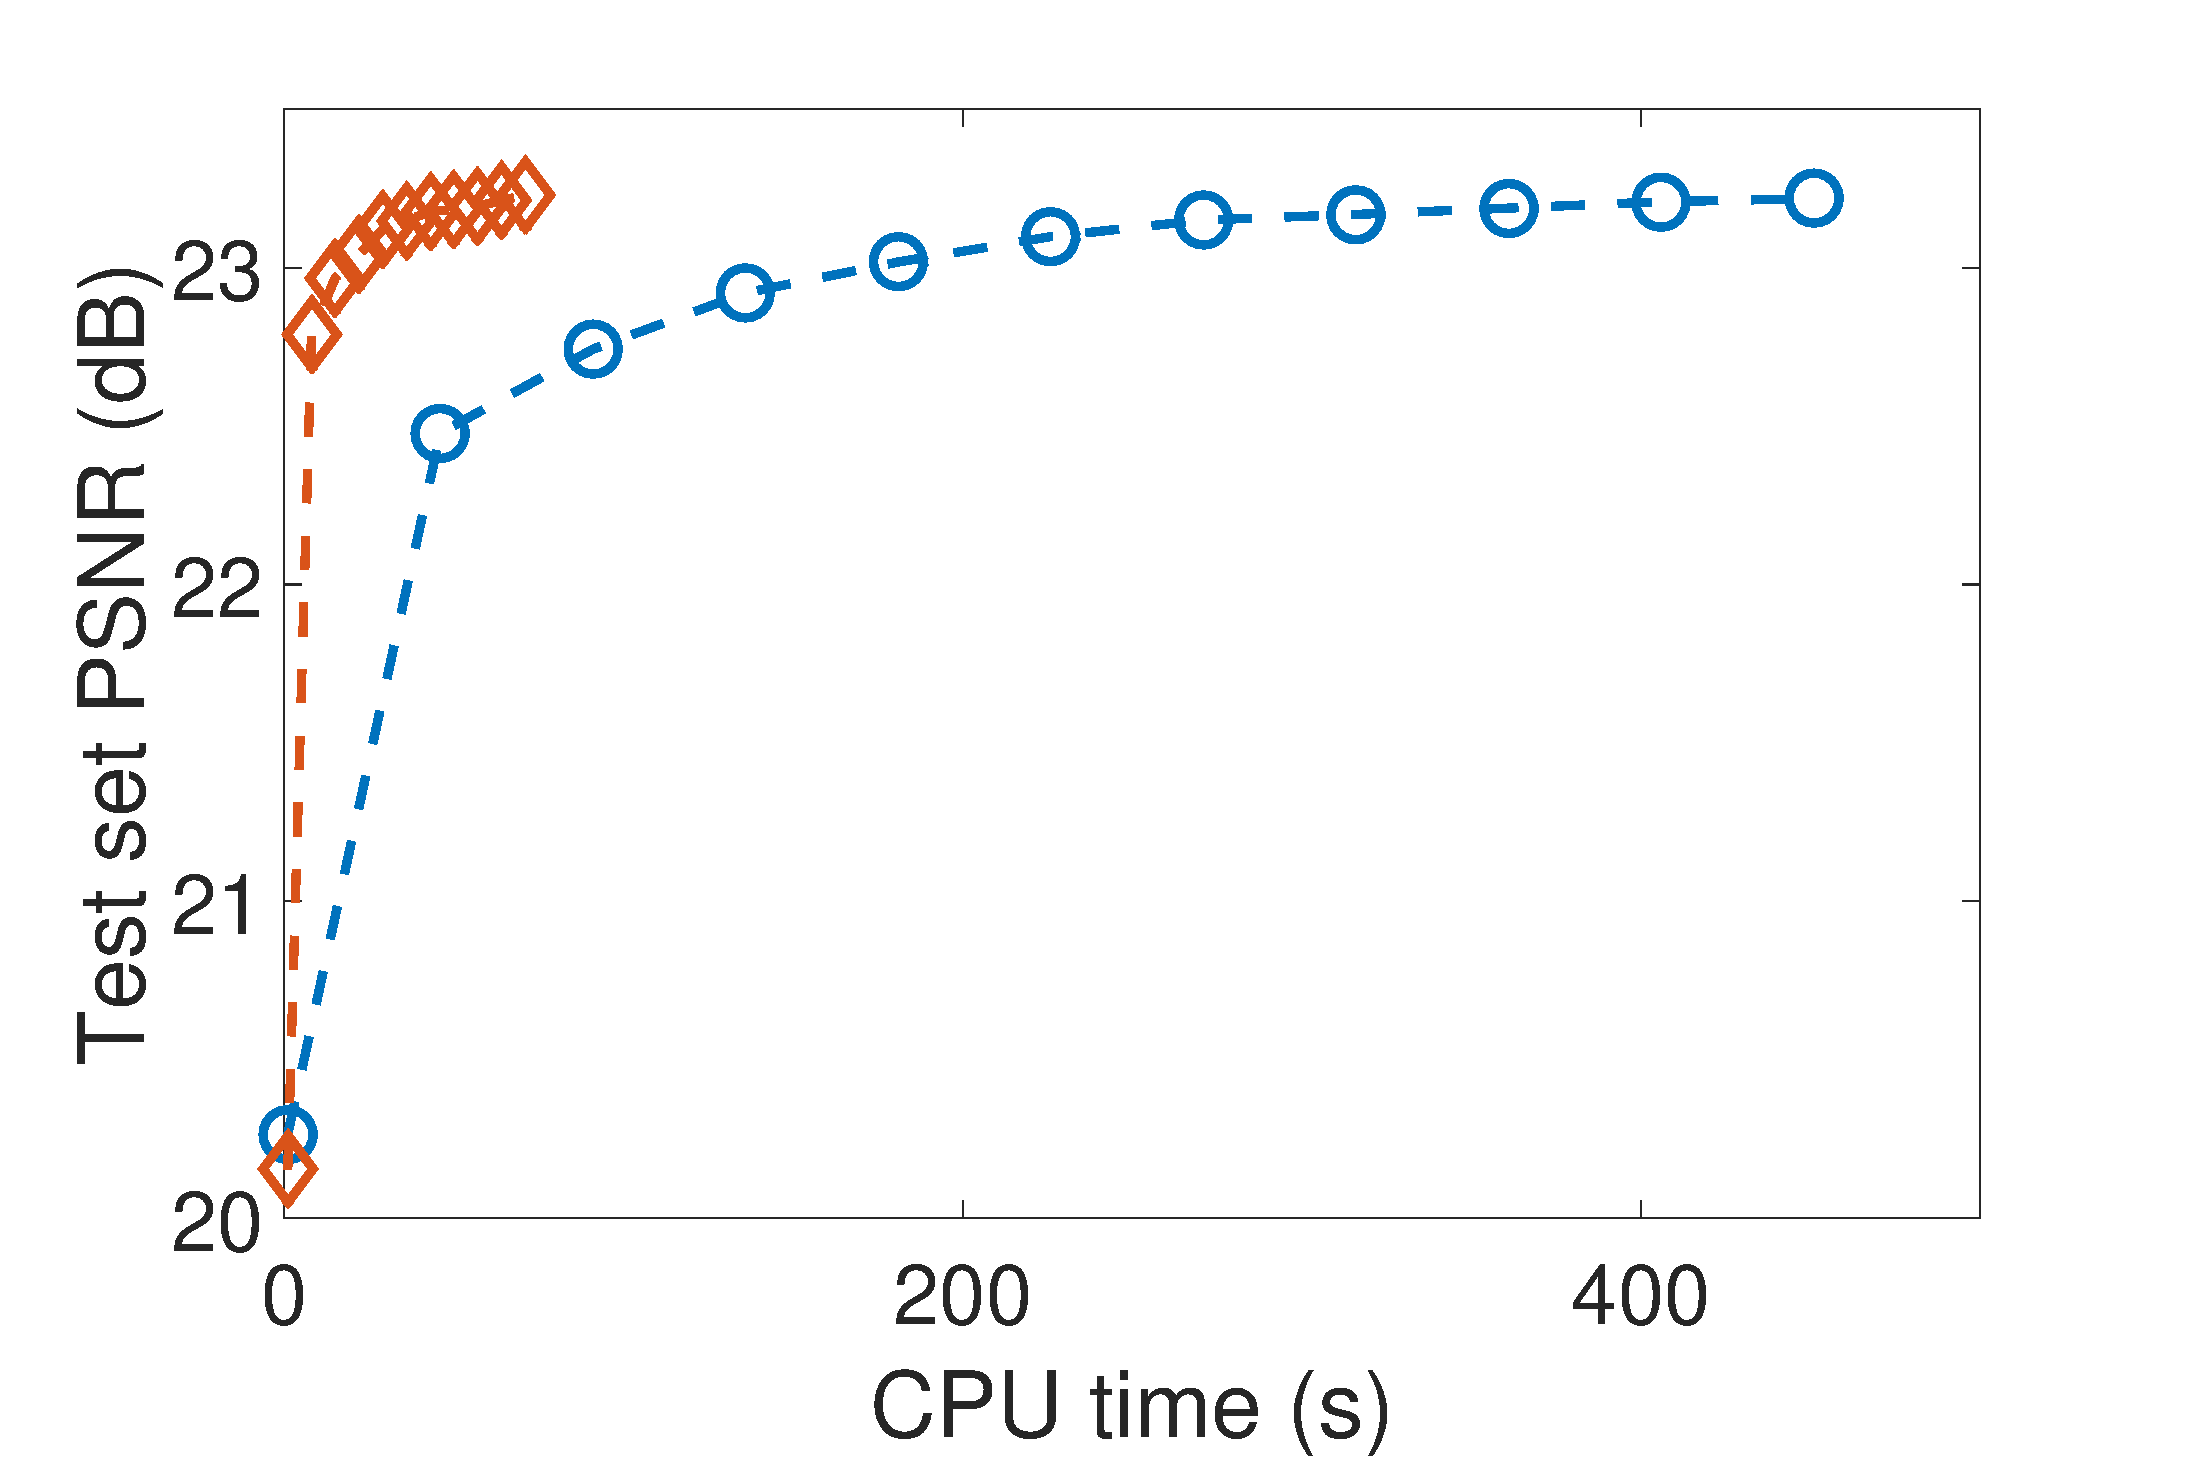
\includegraphics[width=1\linewidth]{figure/onlineVSliu-time-fruit.pdf}
\end{subfigure}

\caption{The experiments are performed on fruit dataset, and each iteration randomly choose one samples from the training datasets. Top: Convergence of the test set objectives (objective value of Eq.~\ref{eq:CSCmodel} on testing datasets) for our method (SOCSC) and the current online approach~\cite{liu-2018-first}. Bottom: Testing PSNR with respect to execution time. While the quality of the output is comparable, our method achieves $6 \times$ speedup.}
\label{fig:onlineSmall}
\end{figure}

{\bfseries Convergence.} Unlike the batch-based learning approaches
which evaluate its convergence by monitoring the objective value on
training datasets, a common way to evaluate the learning process of
online learning model is to monitor its objective value on test
datasets. In Fig.~\ref{fig:onlineSmall} we plot the objective values
against the iteration number for the proposed method (SOCSC) and a
recent online frequency-domain CSC method~\cite{liu-2018-first} (both
 approaches use Matlab built-in functions only). In
the same figure, we also keep track of the capability of the updated
filters during the learning process to sparsely represent the test
images, which is demonstrated by the time evolution of PSNR (PSNR is the 
peak signal-to-noise ratio, measuring the difference between the 
reconstructed signal and the original one). These two
approaches stop at optimum positions with similar objective values.
%although they exhibit slightly different convergence behaviors with
%respect to iterations.
The final PSNR values for both methods also reveal a similar
reconstruction performance of the learned filters. In terms of runtime
comparison, however, the proposed method runs at least $6$ times faster
than the comparison method. Specifically, SOCSC takes 70 seconds and the comparable method takes 440 seconds on a Core i7 PC to process all 10 training images. The supplement shows additional comparisons for the other datasets.

%The proposed method not only exhibits a better convergence performance, but also takes much less execution time, achieving roughly $5 \times$ speedup for one iteration. A visual comparison of the learned dictionaries also demonstrates that the proposed algorithm delivers better outcomes.
% Further numerical comparison will be reported in the next section.

\begin{figure}[h]
\centering
\begin{subfigure}{0.45\textwidth}
  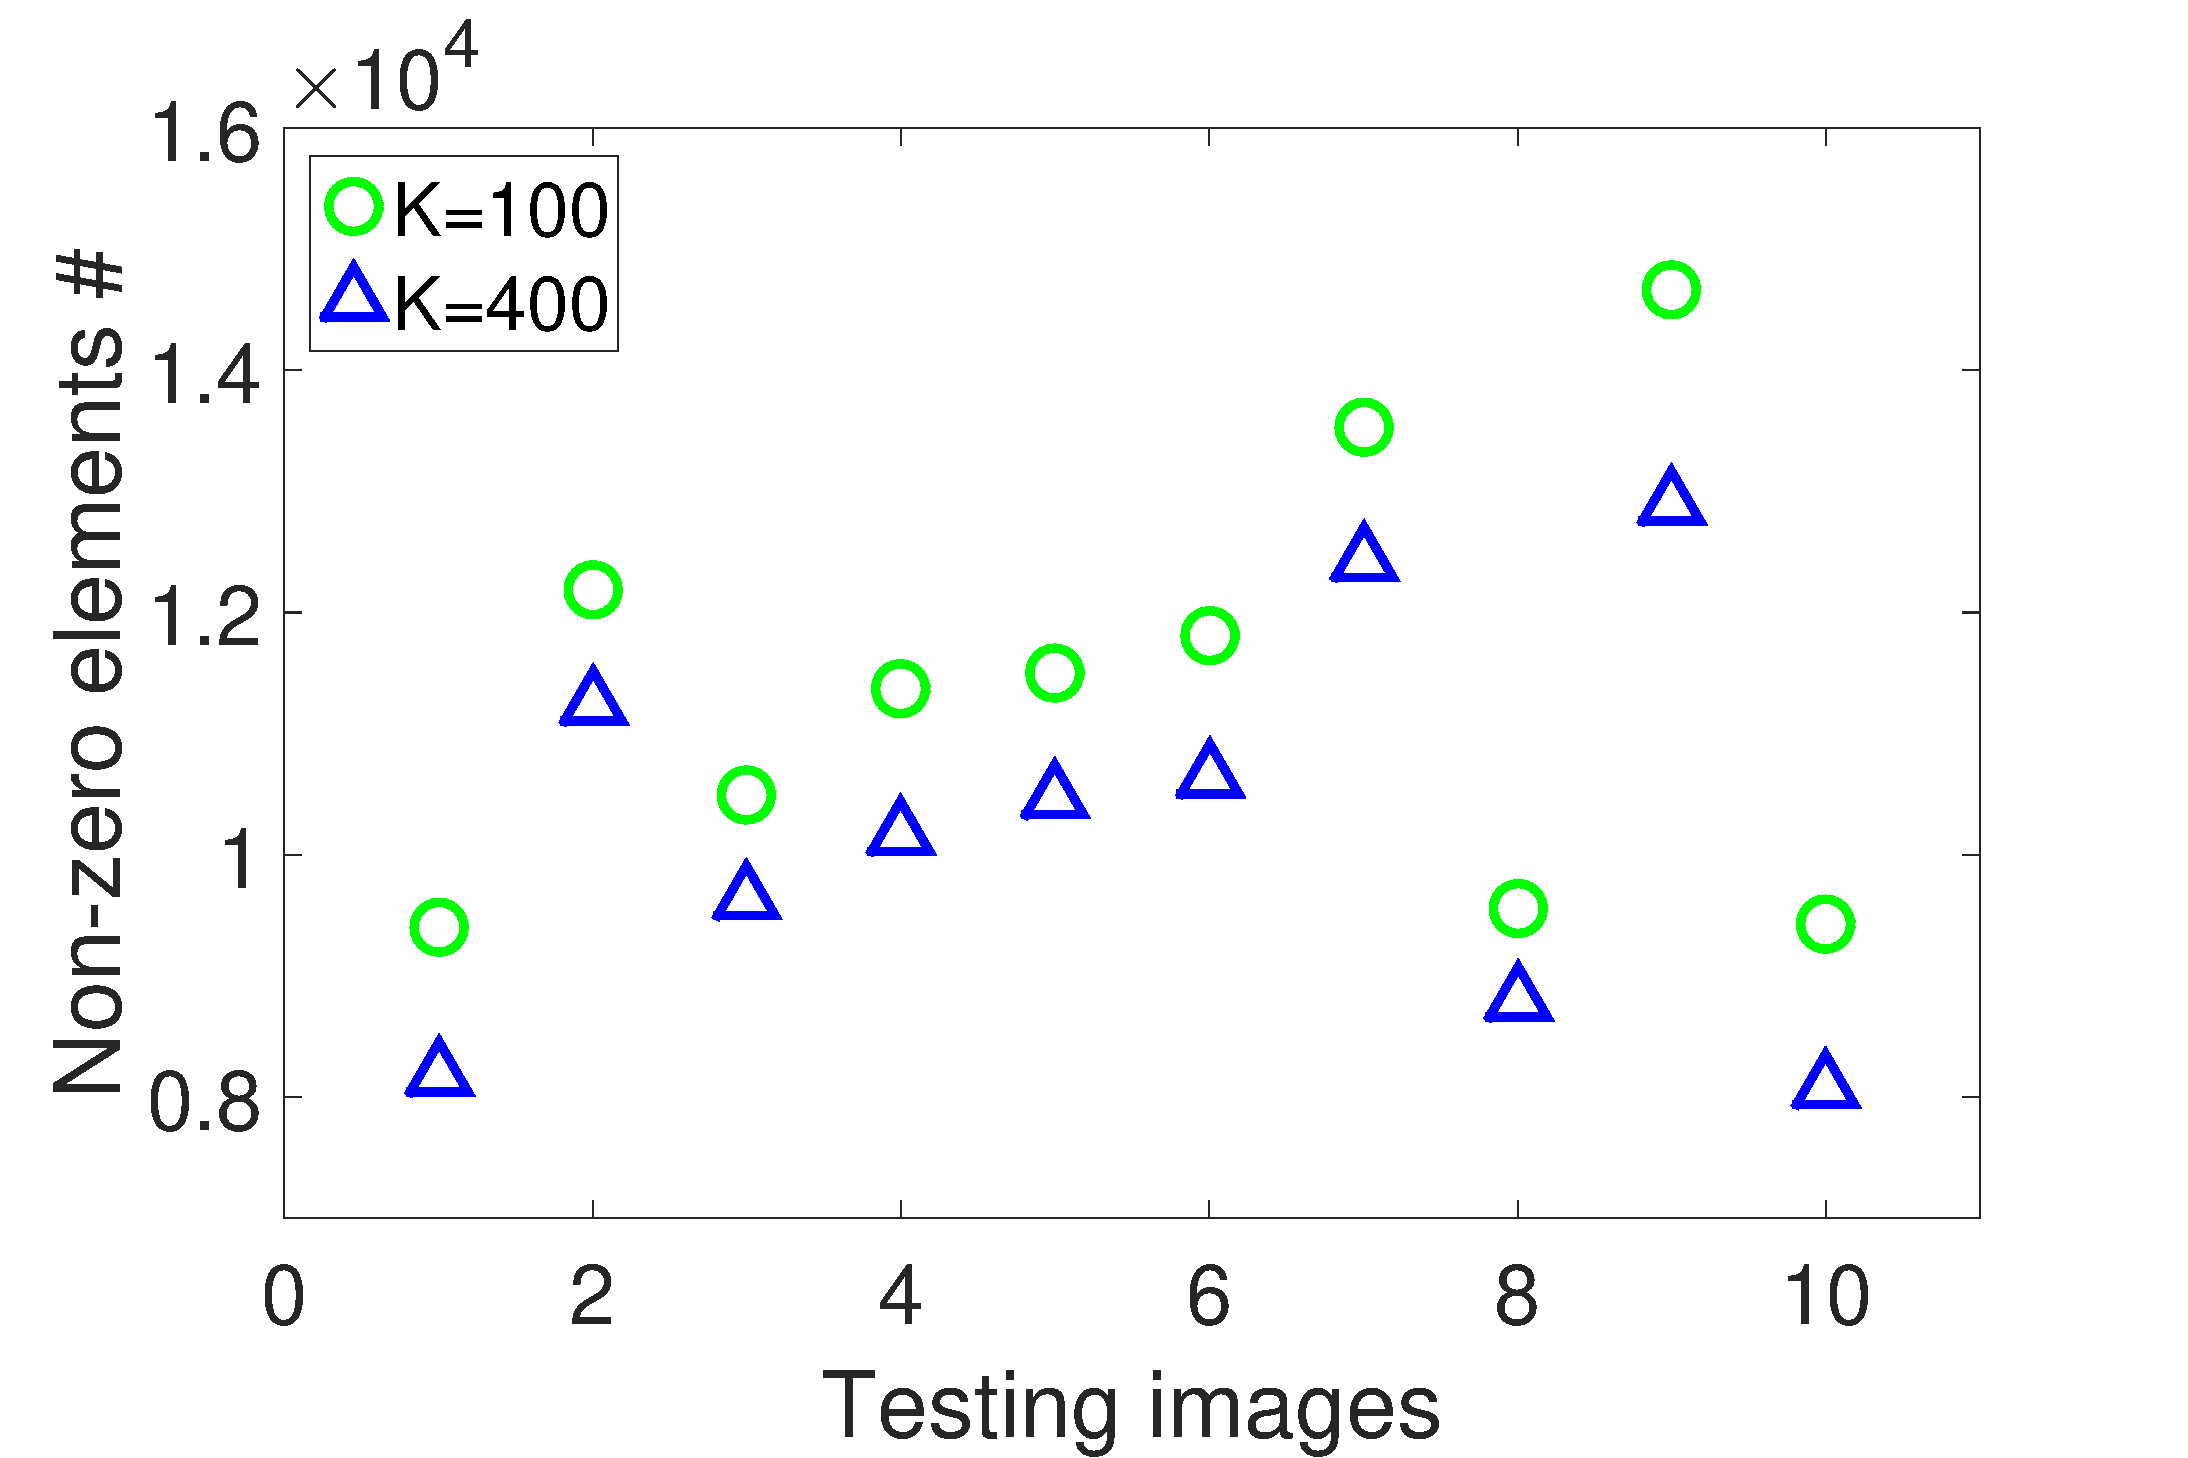
\includegraphics[width=1\linewidth]{figure/nonZeroElement.pdf}
\end{subfigure}
\begin{subfigure}{0.45\textwidth}
  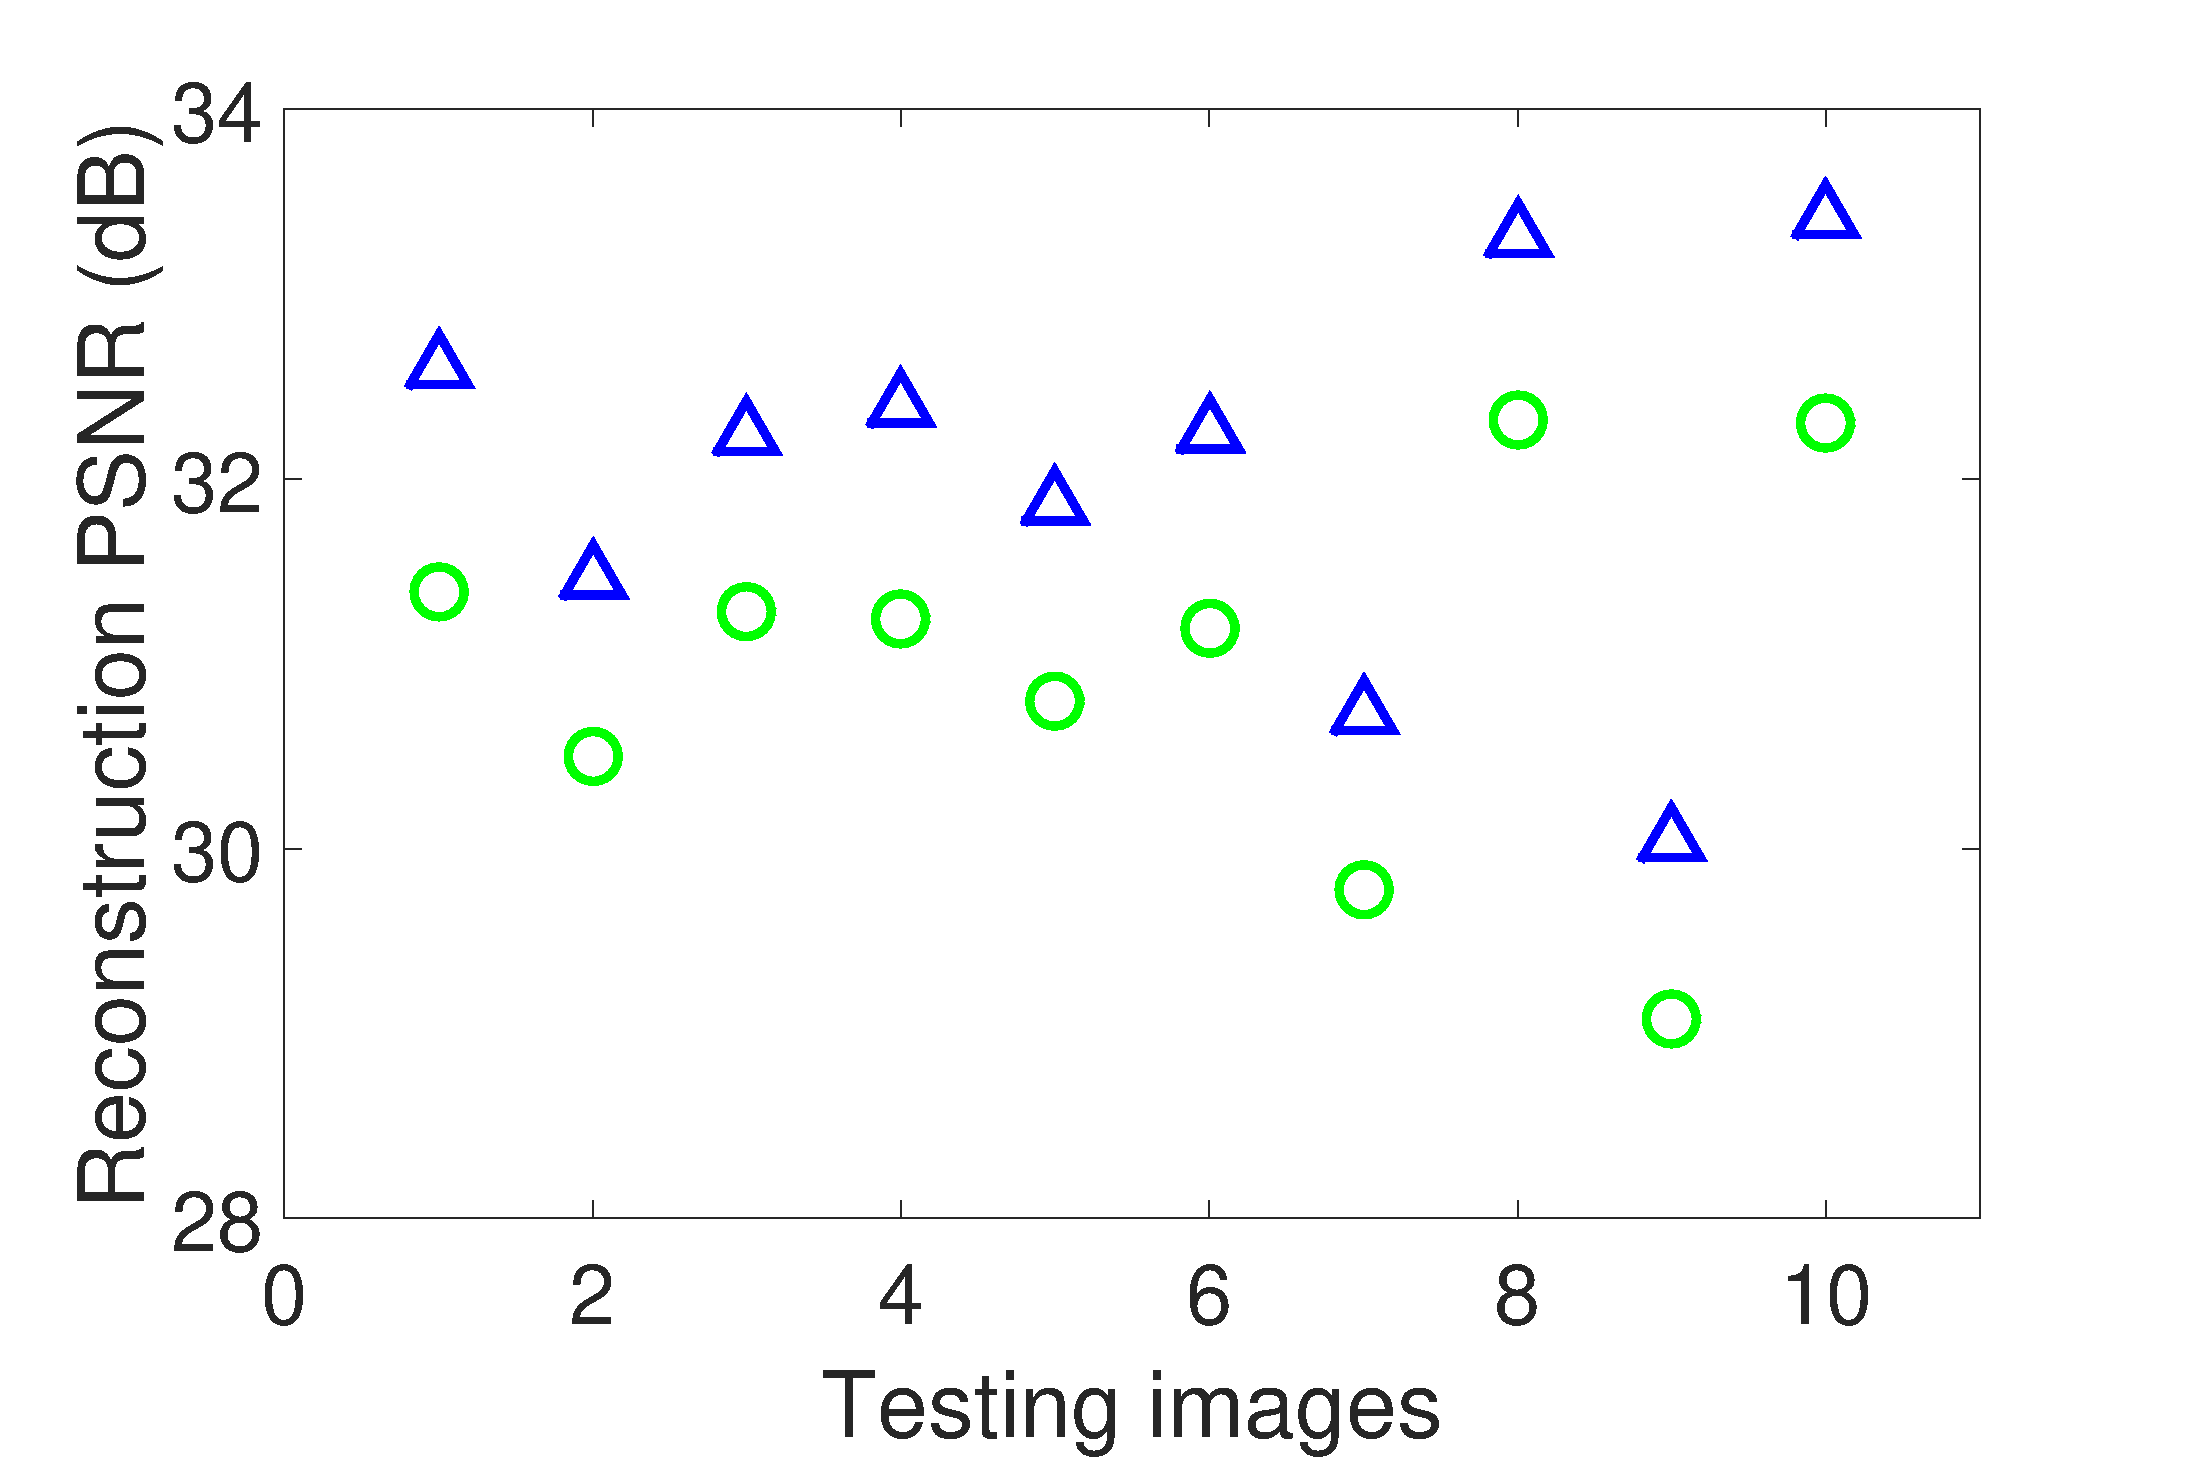
\includegraphics[width=1\linewidth]{figure/reconPSNR.pdf}
\end{subfigure}

\caption{Top: number of non-zero elements in the codes for different images (on average $0.2\%$ of the variables are non-zero when $K=100$). Bottom: PSNR between the reconstructed images and the original ones with under-complete and over-complete dictionaries, respectively.}
\label{fig:overVSunder}
\end{figure}

\begin{figure*}[h]
\begin{minipage}{0.4\textwidth}
\begin{subfigure}{1\textwidth}
    \centering
  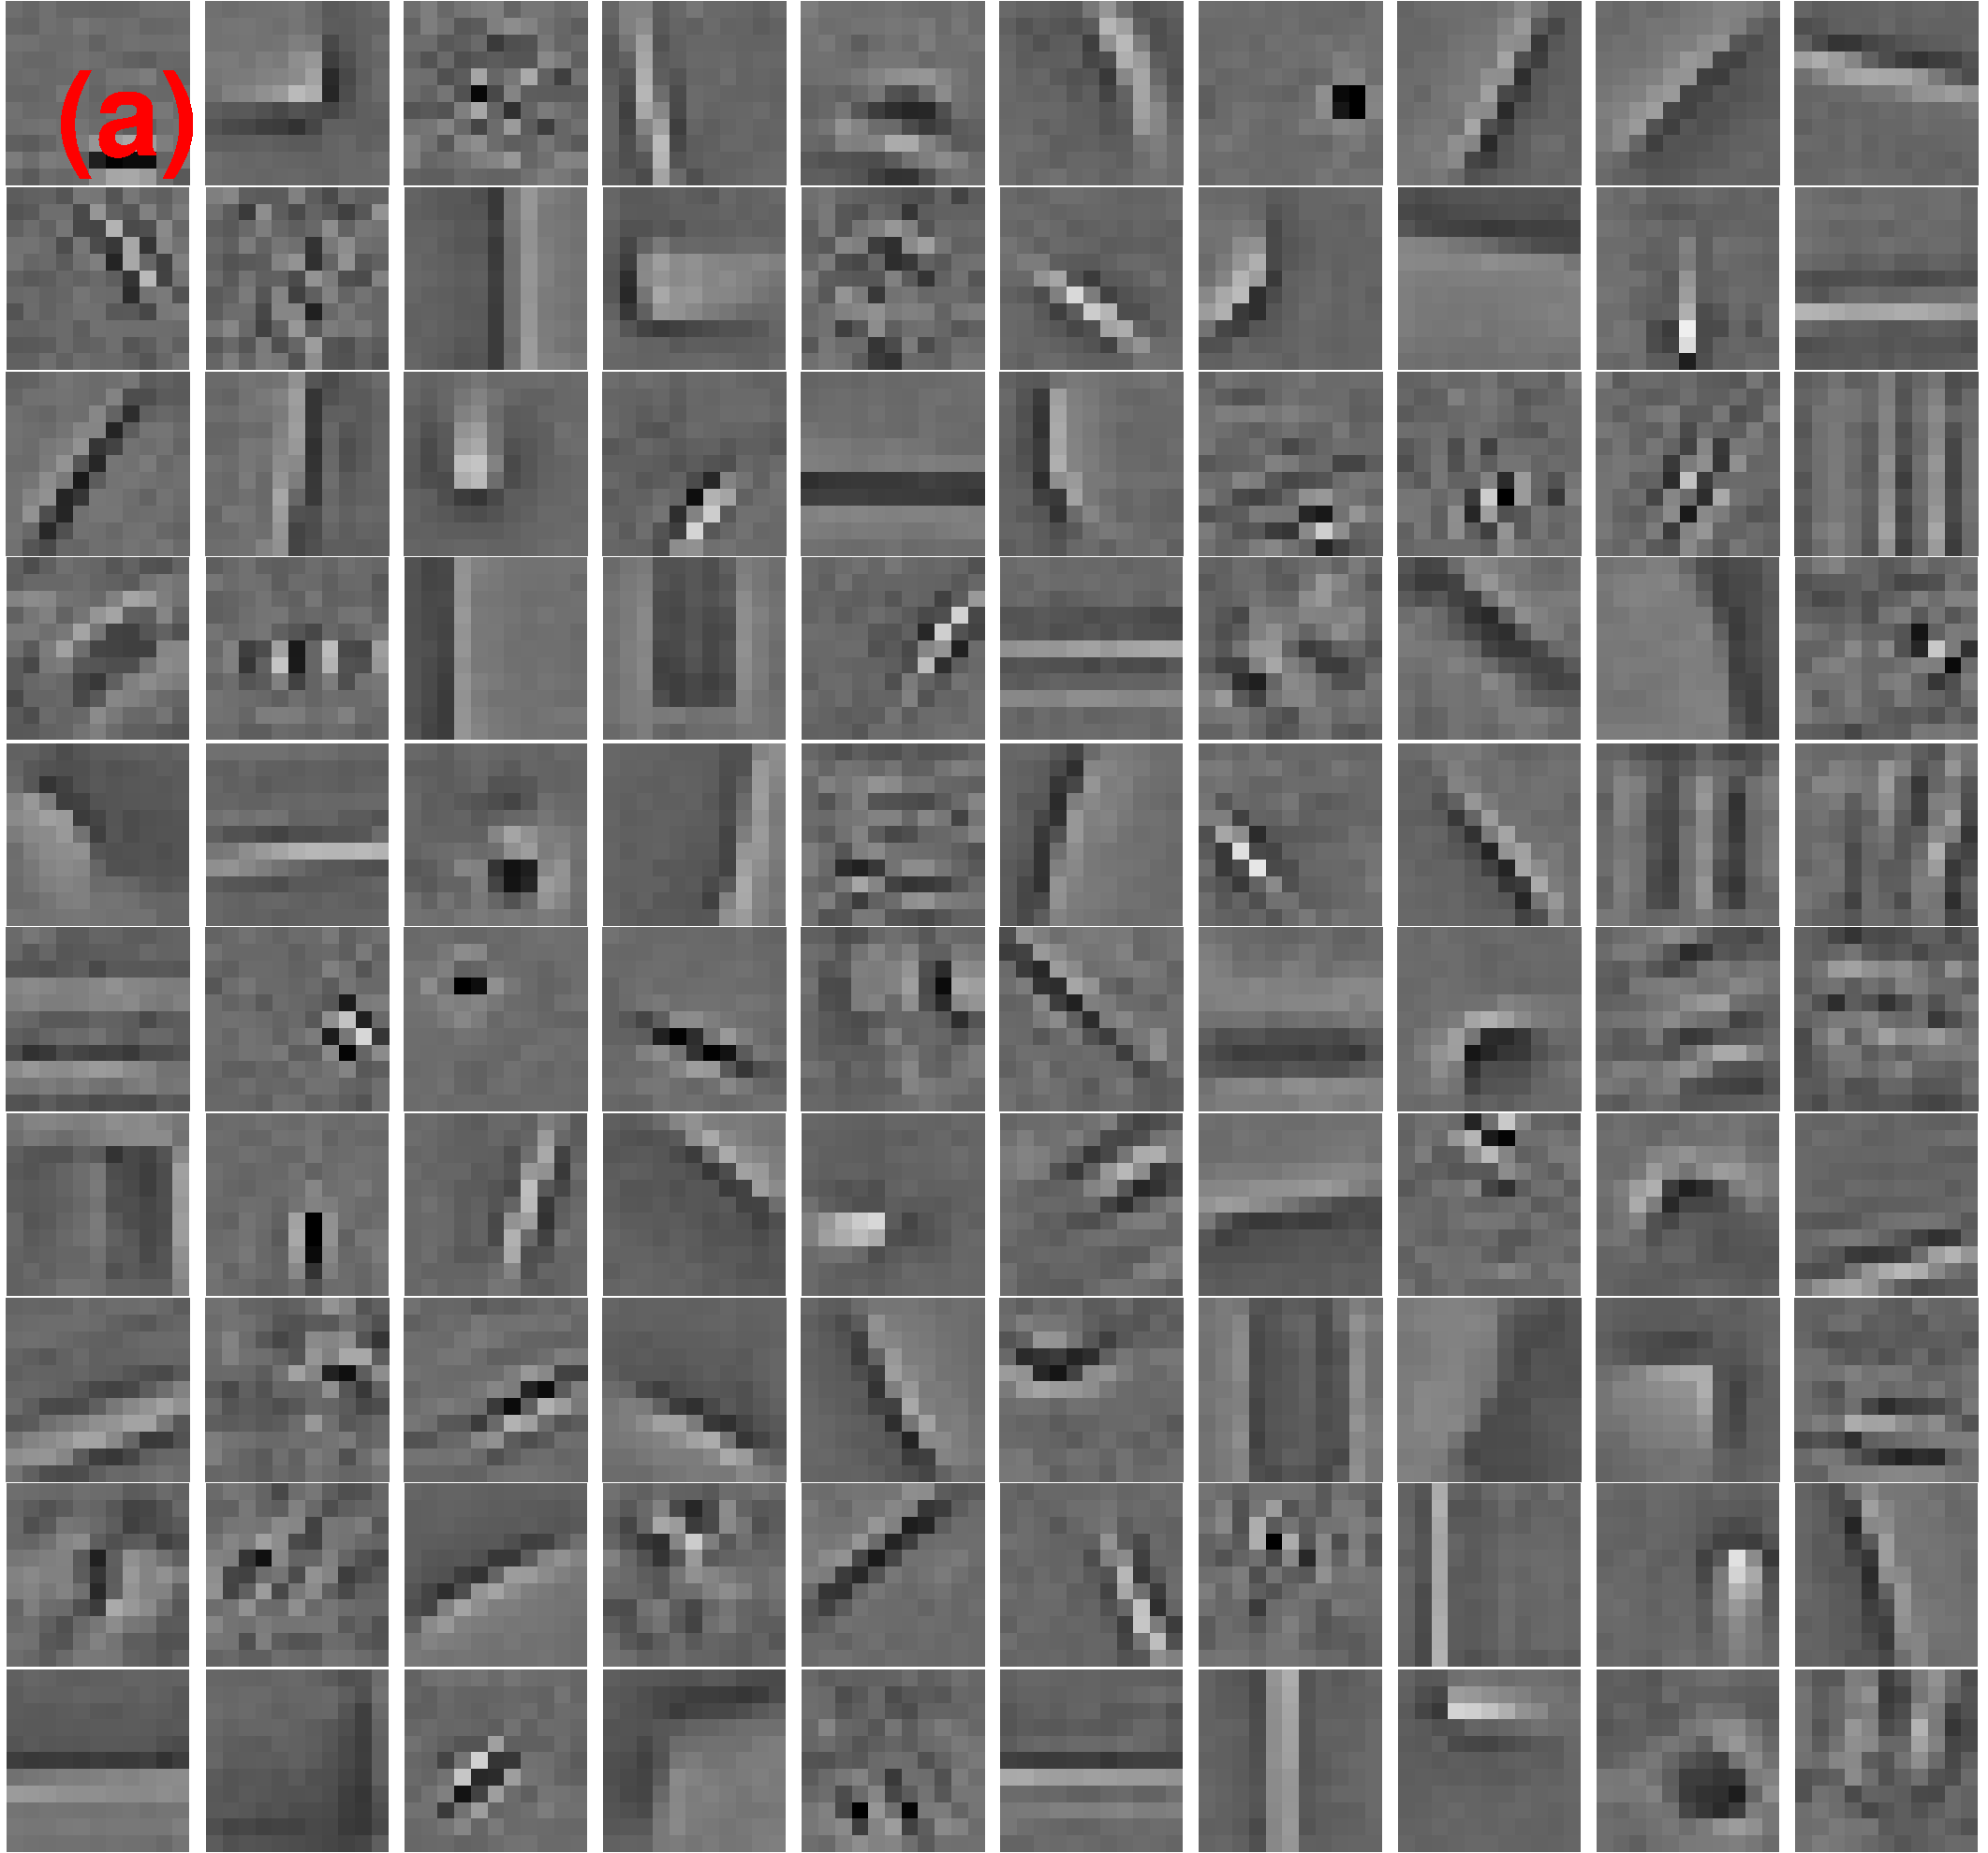
\includegraphics[width=0.75\linewidth]{figure/liu100-filter.pdf}
  \vspace*{2mm}
\end{subfigure}

\begin{subfigure}{1\textwidth}
    \centering
  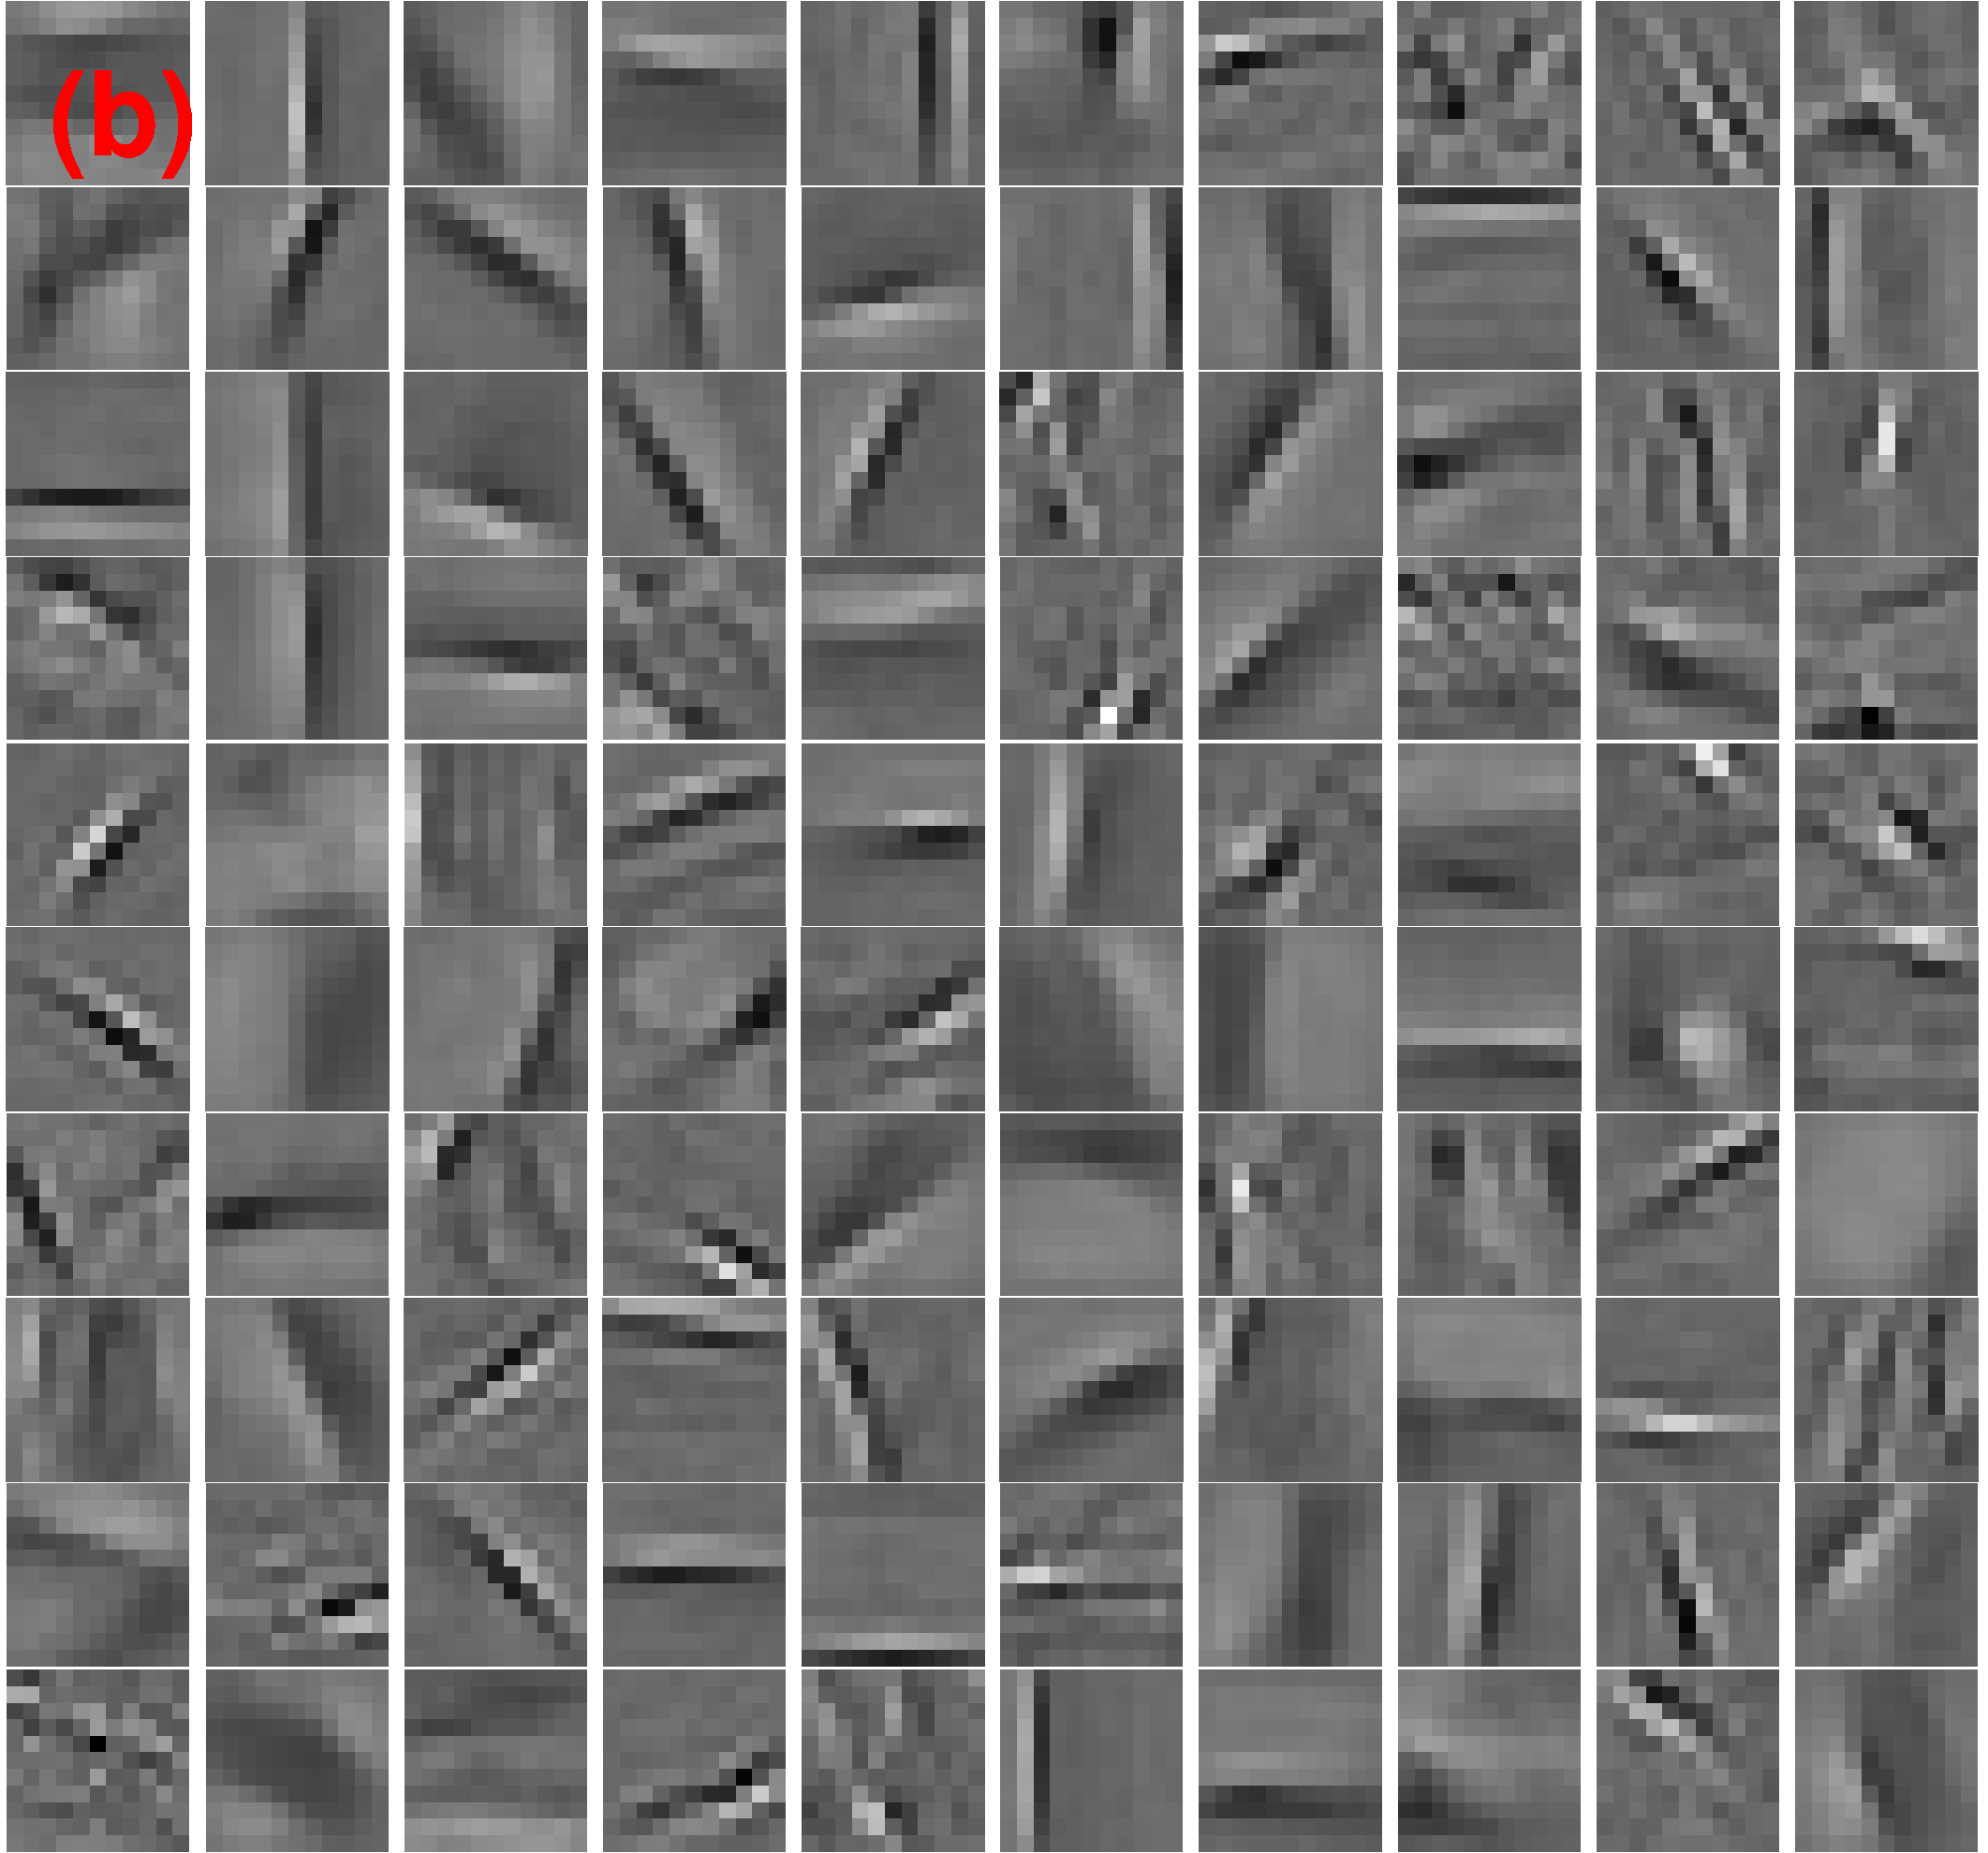
\includegraphics[width=0.75\linewidth]{figure/online100-filter.pdf}
\end{subfigure}
\end{minipage}
\begin{minipage}{0.6\textwidth}
\centering
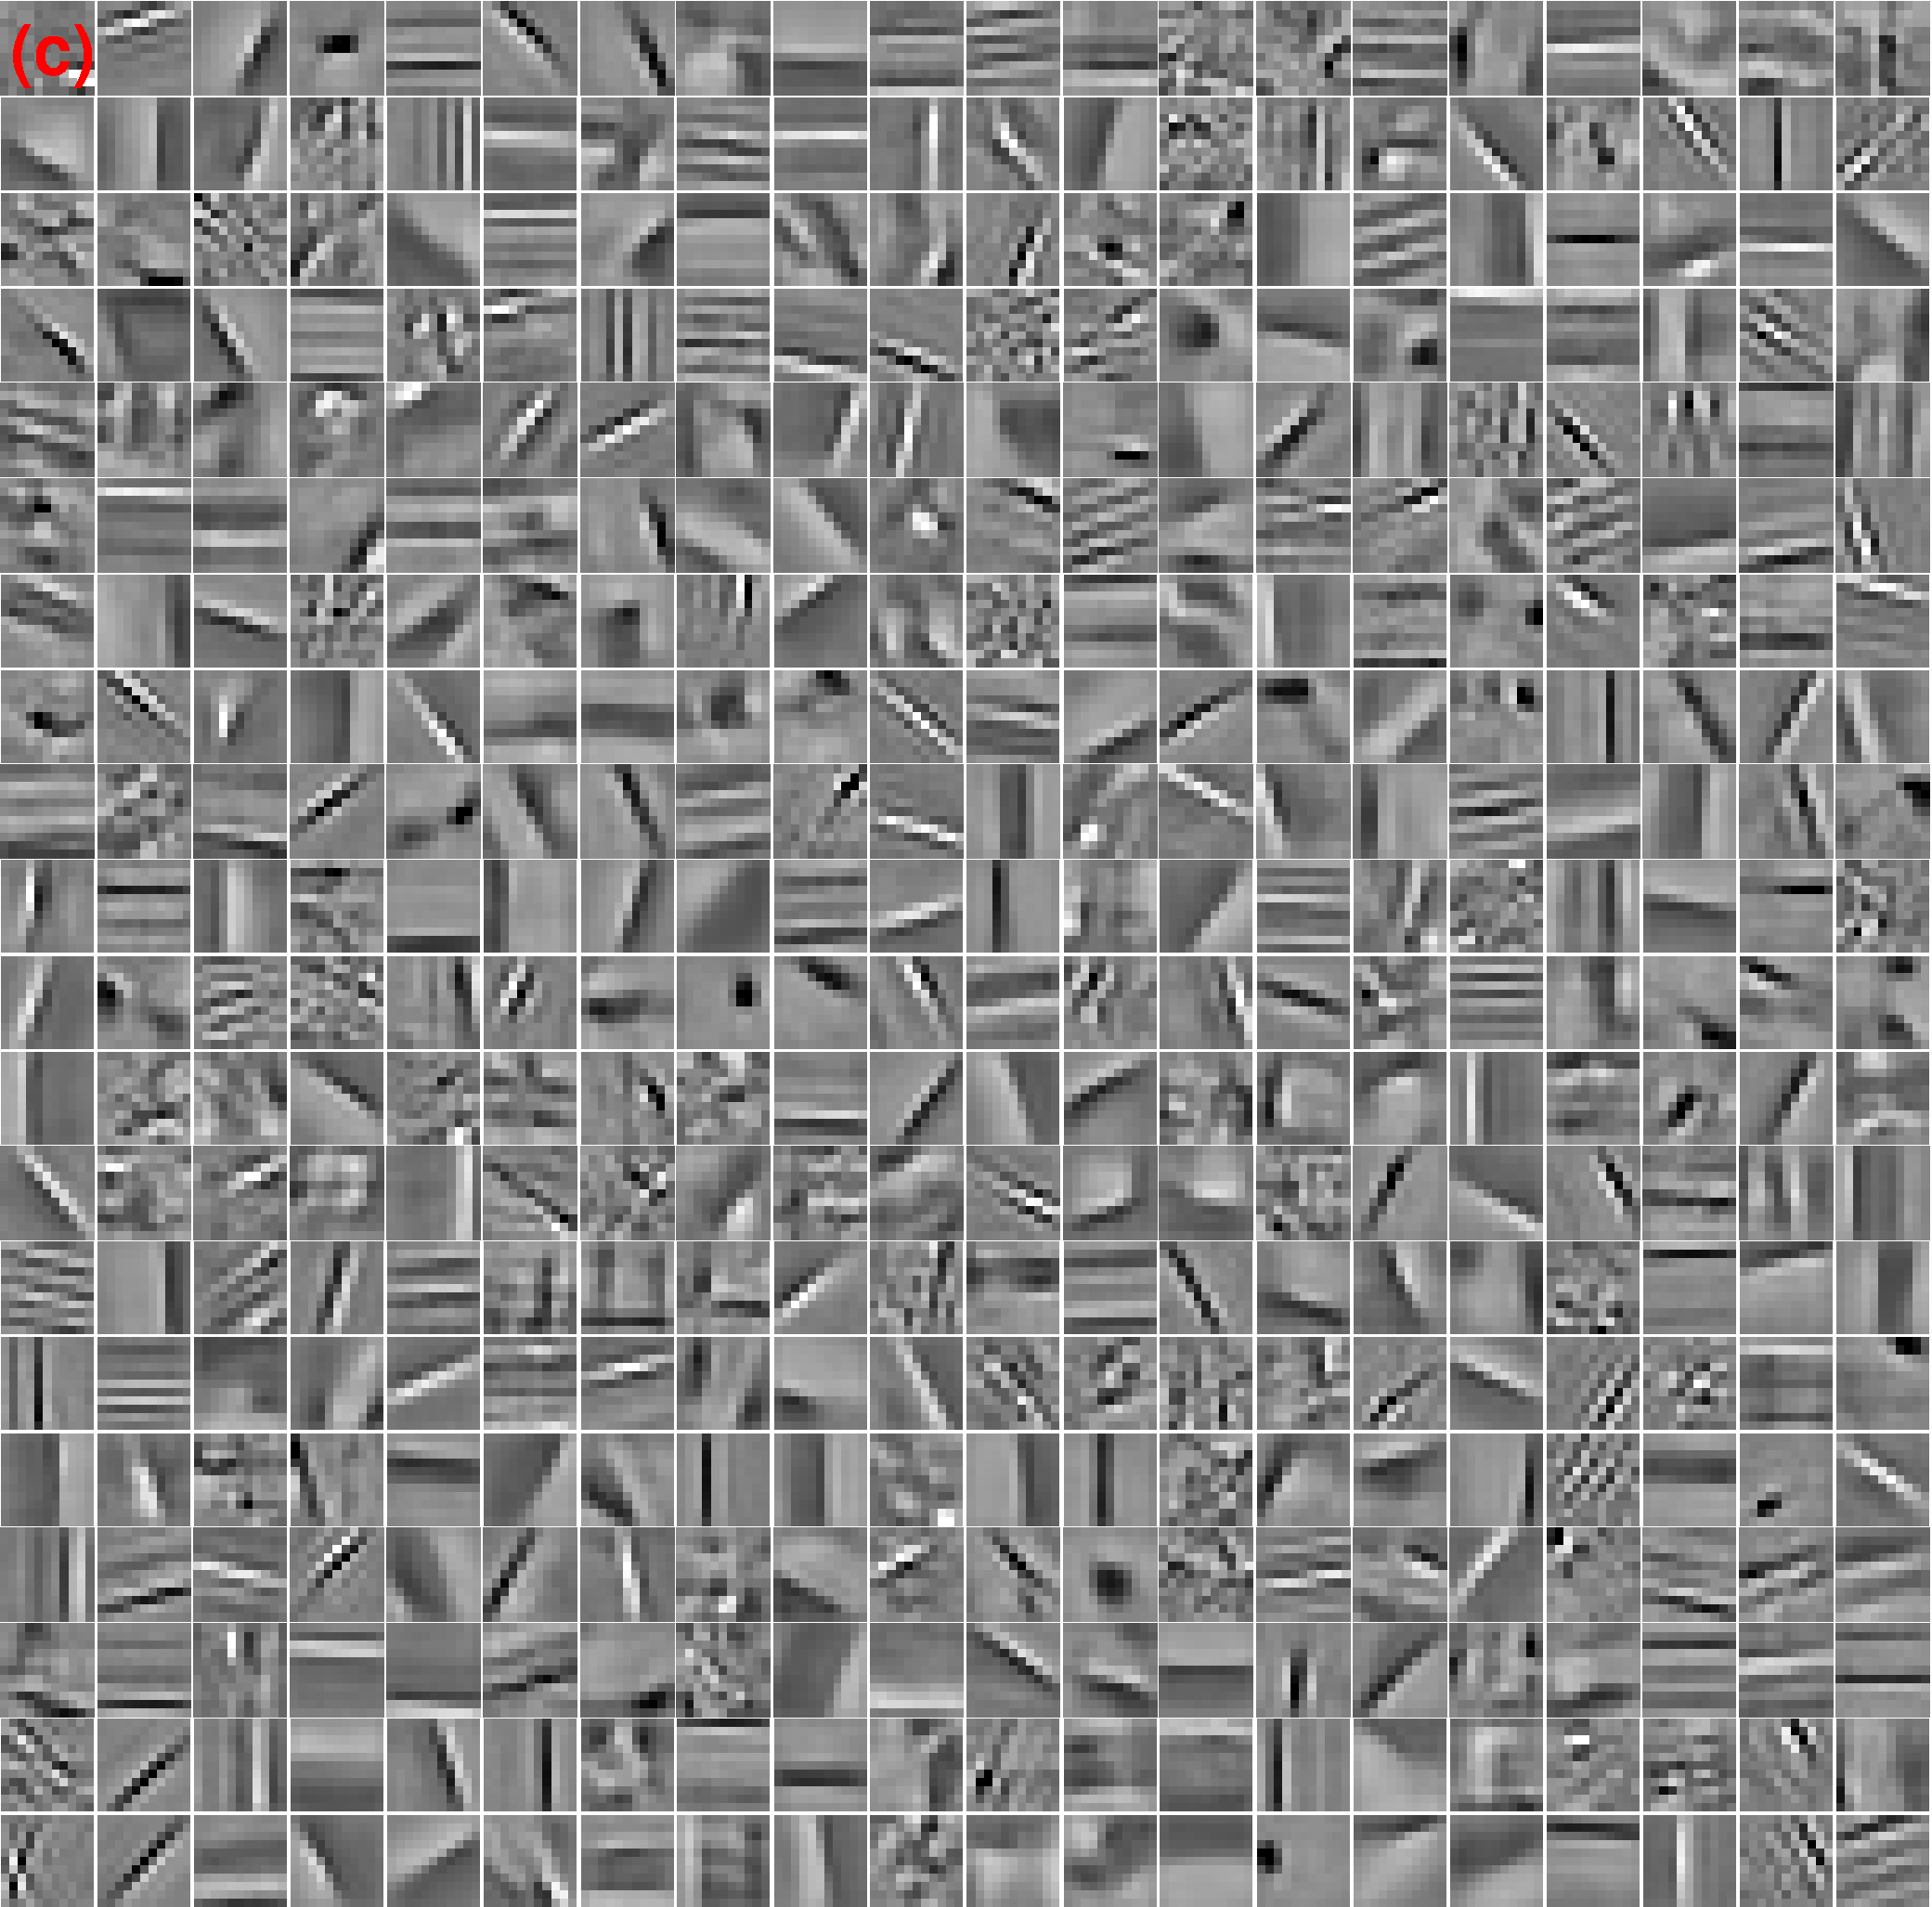
\includegraphics[width=0.97\linewidth]{figure/online400-filter.pdf}
\vspace*{2mm}
\end{minipage}
\begin{minipage}{1\textwidth}
\centering
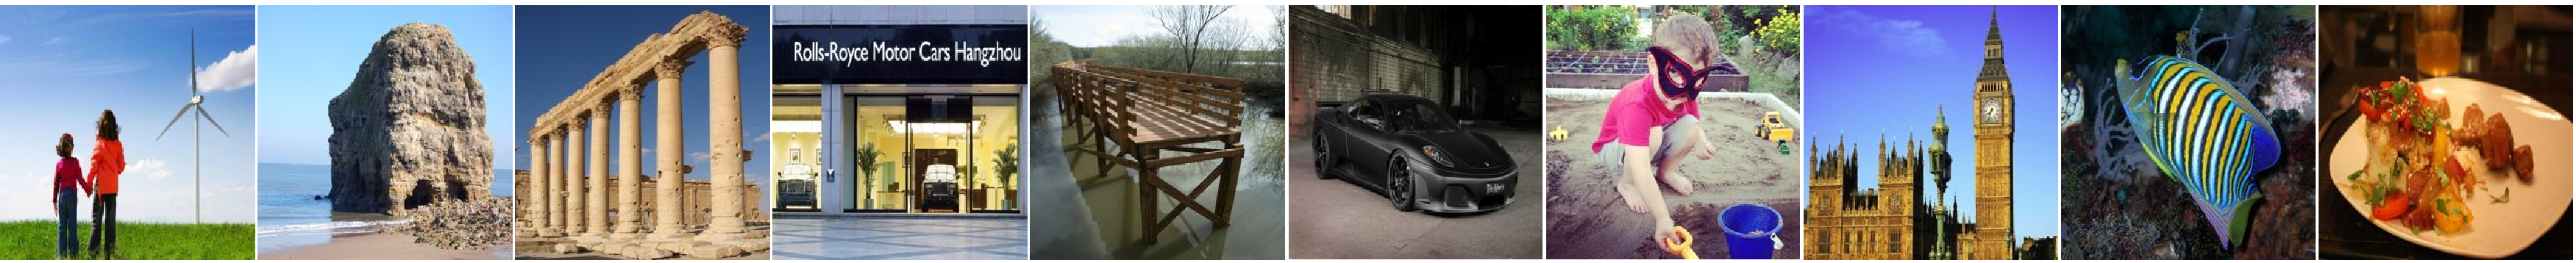
\includegraphics[width=0.9\textwidth]{figure/reconImage.pdf}
\vspace*{2mm}
\end{minipage}
\begin{minipage}{1\textwidth}
    \centering
    \resizebox{0.8\linewidth}{!}{
        \begin{tabular}{|c||c|c|c|c|c|c|c|c|c|c|}
            \cline{1-11}
            Image & 1 & 2 & 3 & 4 & 5 & 6 & 7 & 8 & 9 & 10 \\
            \hline
            PSNR by (a) & 29.58 & 28.19 & 29.44 & 29.63 & 28.89 & 29.33 & 28.13  & 30.14 & 27.42 & 30.89 \\
            \hline
            PSNR by (b) & 29.63 & 28.22 & 29.57 & 29.90 & 29.12 & 29.59 & 28.05  & 30.17 & 27.53 & 31.08 \\
            \hline
            PSNR by (c) & \textbf{30.24} & \textbf{28.34} & \textbf{29.95}  & \textbf{30.30} & \textbf{29.43} & \textbf{29.96} & \textbf{28.24} & \textbf{30.57} & \textbf{27.72} & \textbf{31.67} \\
            \hline
        \end{tabular} }
\end{minipage}
\caption{Top: Filters learned from large-scale datasets by our method (SOCSC) and the comparable online method~\cite{liu-2018-first}. Bottom: $10 ~ 256 \times 256$ testing images and their corresponding reconstruction quality in the image inpainting application. (a) The under-complete dictionary ($11 \times 11 \times 100$) learned by~\cite{liu-2018-first}; (b) The under-complete dictionary ($11 \times 11 \times 100$) learned by SOCSC. (c) The over-complete dictionary ($11 \times 11 \times 400$) learned by SOCSC. These under-complete dictionaries, mainly composed of Gabor-like filters, can be seen as a subset of the represented over-complete dictionary, which contains a number of extra low contrast image features.}
\label{fig:overCompleteDic}
\end{figure*}

{\bfseries Over-complete dictionary.}
%To our knowledge, none of the
%existing CSC work reported or analyzed the over-complete dictionary
%(number of the dictionary is more than its degrees of freedom). One of
%the reasons could be that most of the prior work is batch-based, thus
%learning over-complete dictionary from small datasets would cause
%overfitting issues, which may contain quite a few data-specific
%filters, and therefore limit the ability to generalize the filters to
%other data (we verify this explanation in the supplement). The
%proposed online-based learning strategy (SOCSC) can overcome this
%issue by scaling the model up to arbitrary sample sizes.
Learning over-complete dictionary (number of the dictionary is more
than its degrees of freedom) from small datasets would cause
overfitting issues, which may contain quite a few data-specific
filters, and therefore limit the ability to generalize the filters to
other data (we verify this explanation in the supplement). The
proposed online-based learning strategy (SOCSC) can overcome this
issue by scaling the model up to arbitrary sample sizes.

We demonstrate this ability on 1000 image patches with the size of
$100 \times 100$, and learn an $11 \times 11 \times 400$ over-complete
dictionary, which is shown in Fig.~\ref{fig:overCompleteDic}. For a
visual comparison, we also show $100$ learned filters generated by the
same algorithm and another 100 filters generated
by~\cite{liu-2018-first}. As can be observed, both of the approaches
learn visually similar under-complete dictionary, while the proposed
method takes $6 \times$ less training time than the comparison
method. The learned over-complete dictionary is composed of
the Gabor-like image features as represented in the under-complete
dictionaries, as well as a number of low contrast features which are
not typical for under-complete dictionaries. This additional
feature information would play an essential role to reveal an improved sparse representation of
the natural images. The numerical comparisons of number of non-zero elements and its corresponding reconstruction PSNR for testing images ($10 ~ 256 \times 256$ images presented in Fig.~\ref{fig:overCompleteDic}) are shown in Fig.~\ref{fig:overVSunder}. Here, we define the non-zero elements as the codes whose coefficient is no less than $0.1$. We could observe that at all times, using over-complete dictionary leads to a sparser representation of the images, roughly $8\%-10\%$ reduction on the non-zero elements. Meanwhile, it achieves dramatically improved reconstruction quality, over $1$ dB on average.

We further demonstrate the effectiveness of the over-complete
dictionary in the application of image inpainting,
which refers to reconstructing a full image from partial
measurements. A numerical comparison of the reconstruction quality is
shown in the bottom of Fig.~\ref{fig:overCompleteDic}. The reconstructions
are performed on $50\%$ randomly observed images, with $\lambda = 0.4$ and
$50$ ADMM iterations for all cases. Obtained PSNR values are averaged on
5 trials. The over-complete filters learned by the proposed
method achieves significantly improved reconstruction quality on partially 
observed images in terms of the PSNR value.

We also observe a bottleneck revealed by the under-complete dictionary
in the online-based CSC model. The top of Fig.~\ref{fig:overComDicAndMinibatch} demonstrates that no more
apparent progress could be observed when the number of training images
is higher than a specific value for both of the online approaches
($K=100$). However, owing to more abundant filters, learning
over-complete dictionary overcomes this bottleneck, and it shows a
considerable improvement in the PSNR of image representations. All 
presented experimental results imply that the number of filters and 
number of training samples are both essential in the CSC model.

{\bfseries Mini-batching.} In practice, a mini-batching strategy would
be preferred in order to gain advantages from modern parallel
computing architectures. This is also a standard extension to
stochastic optimization algorithms~\cite{Takac2013, PCDM, SCSG}. We
denote the mini-batch size as $\eta$. In the proposed online algorithm
(SOCSC), the time complexity for one step dictionary update will not
increase linearly with the increase of $\eta$. Concretely speaking,
updating $\code$ can be implemented by caching the Cholesky
decomposition, and one computation of the matrix factorization can be
applied to all of the currently selected batches. Herein, the
complexity for doing updating $\code$ $\eta$ times all together is
cheaper than $\eta$ times the complexity of updating one $\code$. In
addition, the time complexity for updating $\filter$ is not linearly
affected by the value of $\eta$, which will be executed only once in
each training step regardless of $\eta$. One exception is the update
of surrogate matrices which has a complexity that is linear in
$\eta$. However, this step is not dominant in the runtime.

\begin{figure}[h]
\centering
\begin{subfigure}{0.45\textwidth}
  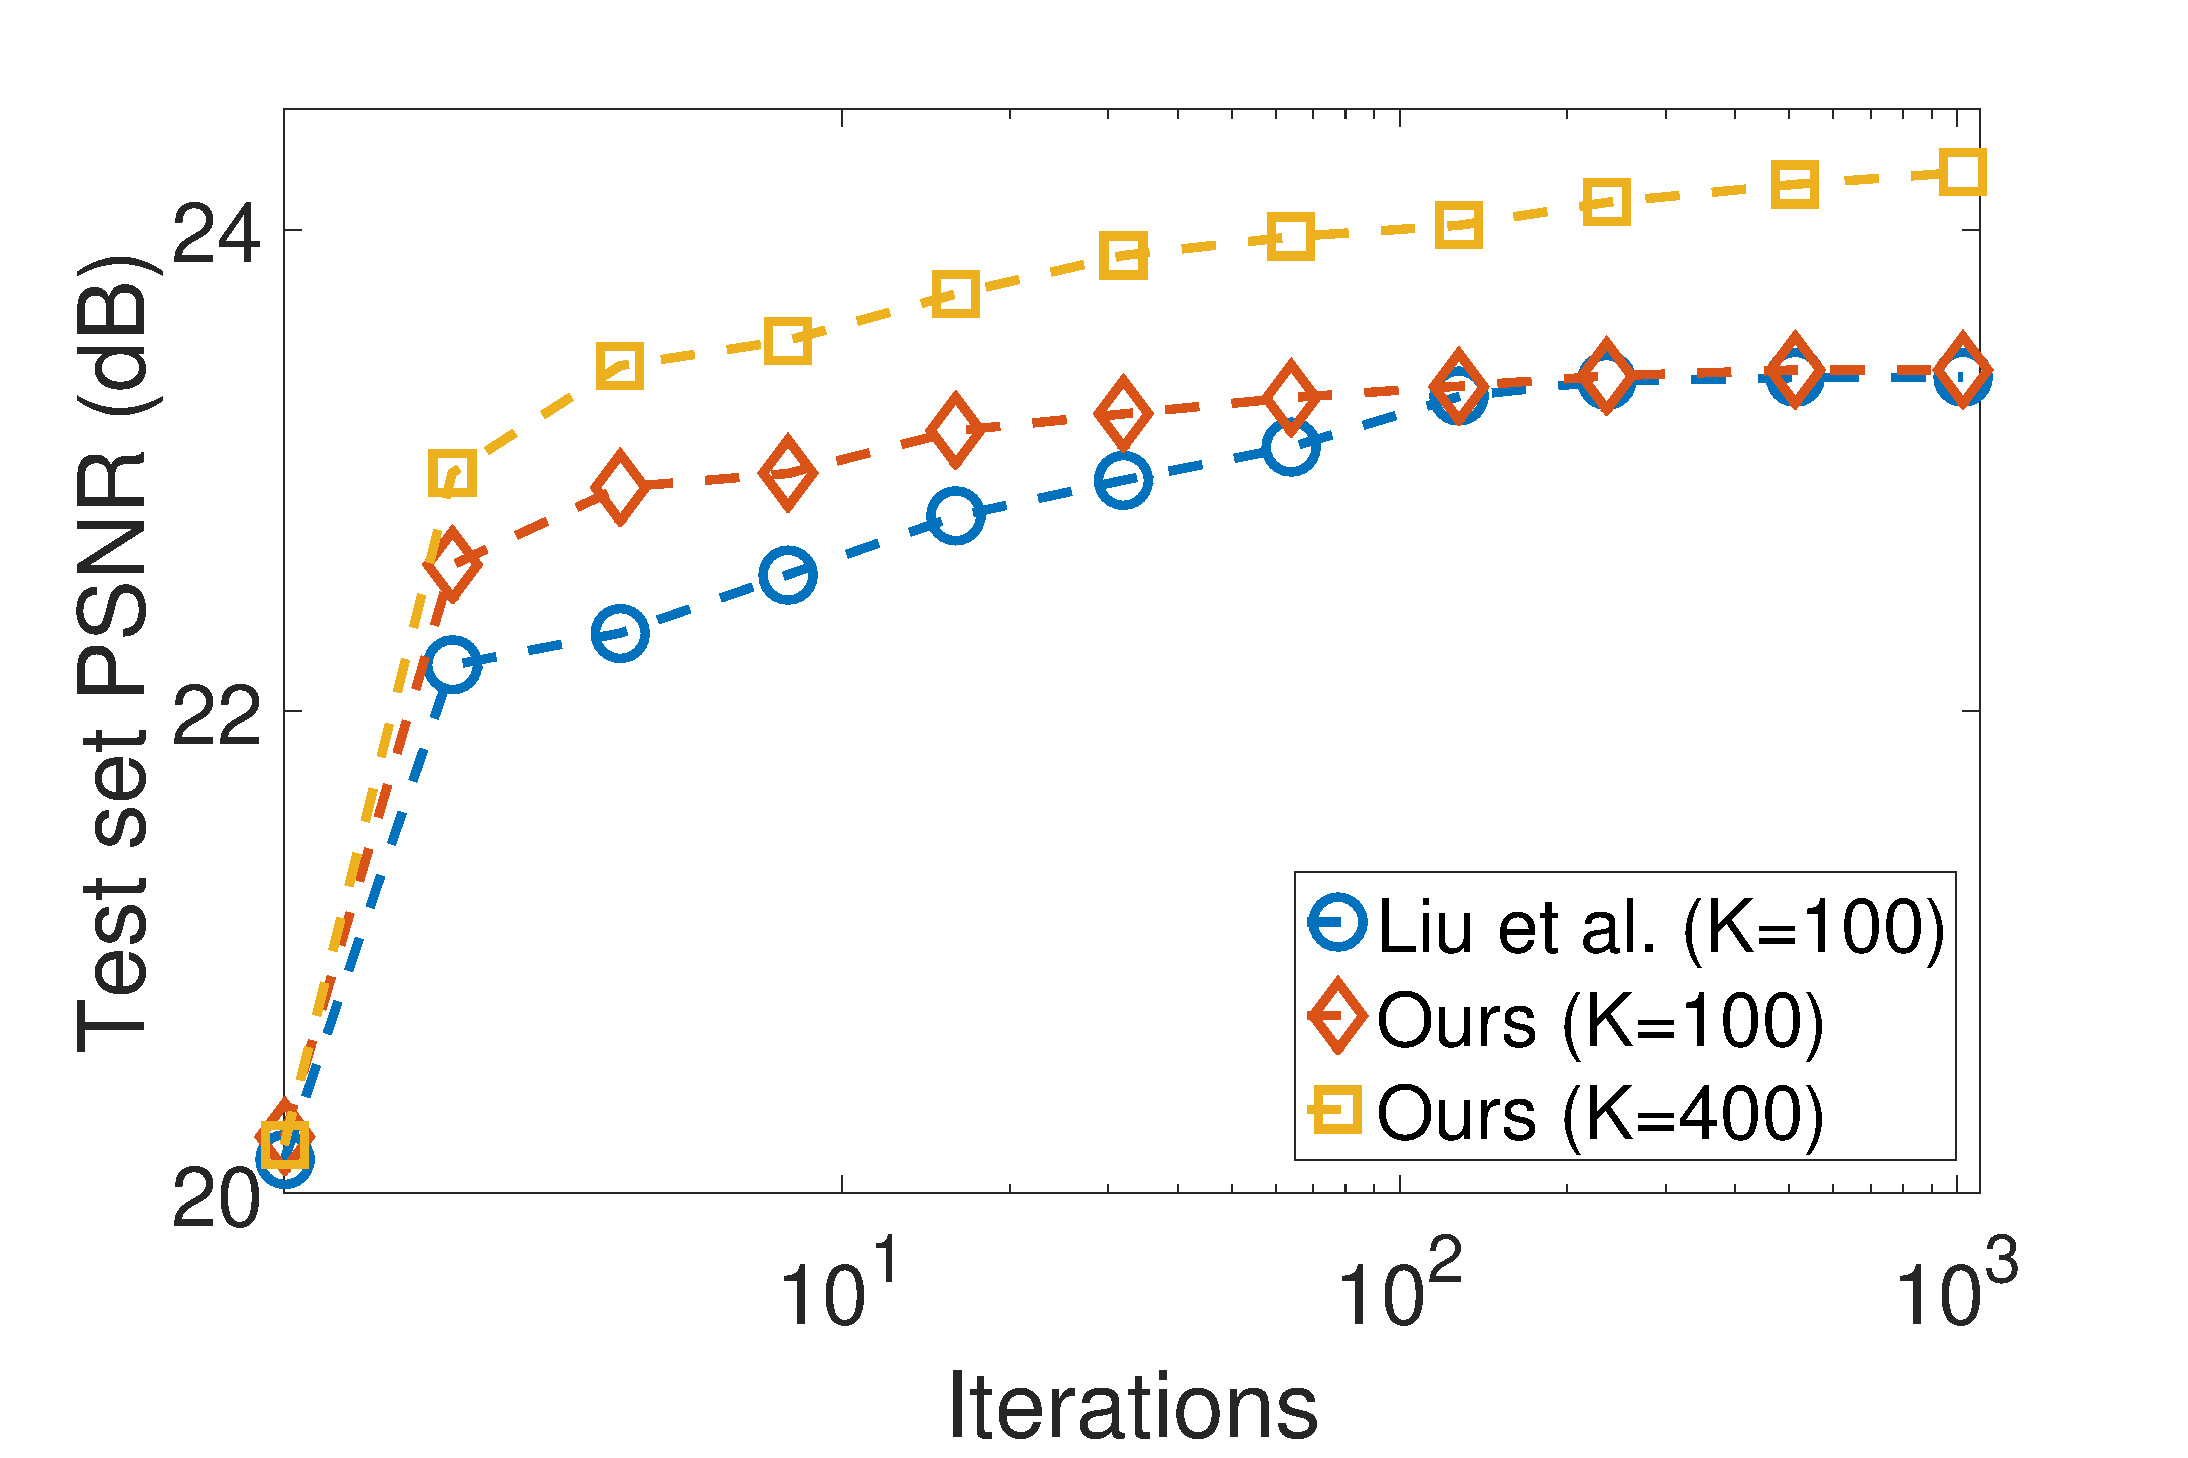
\includegraphics[width=1\linewidth]{figure/overComplete-ite.pdf}
\end{subfigure}
\begin{subfigure}{0.45\textwidth}
  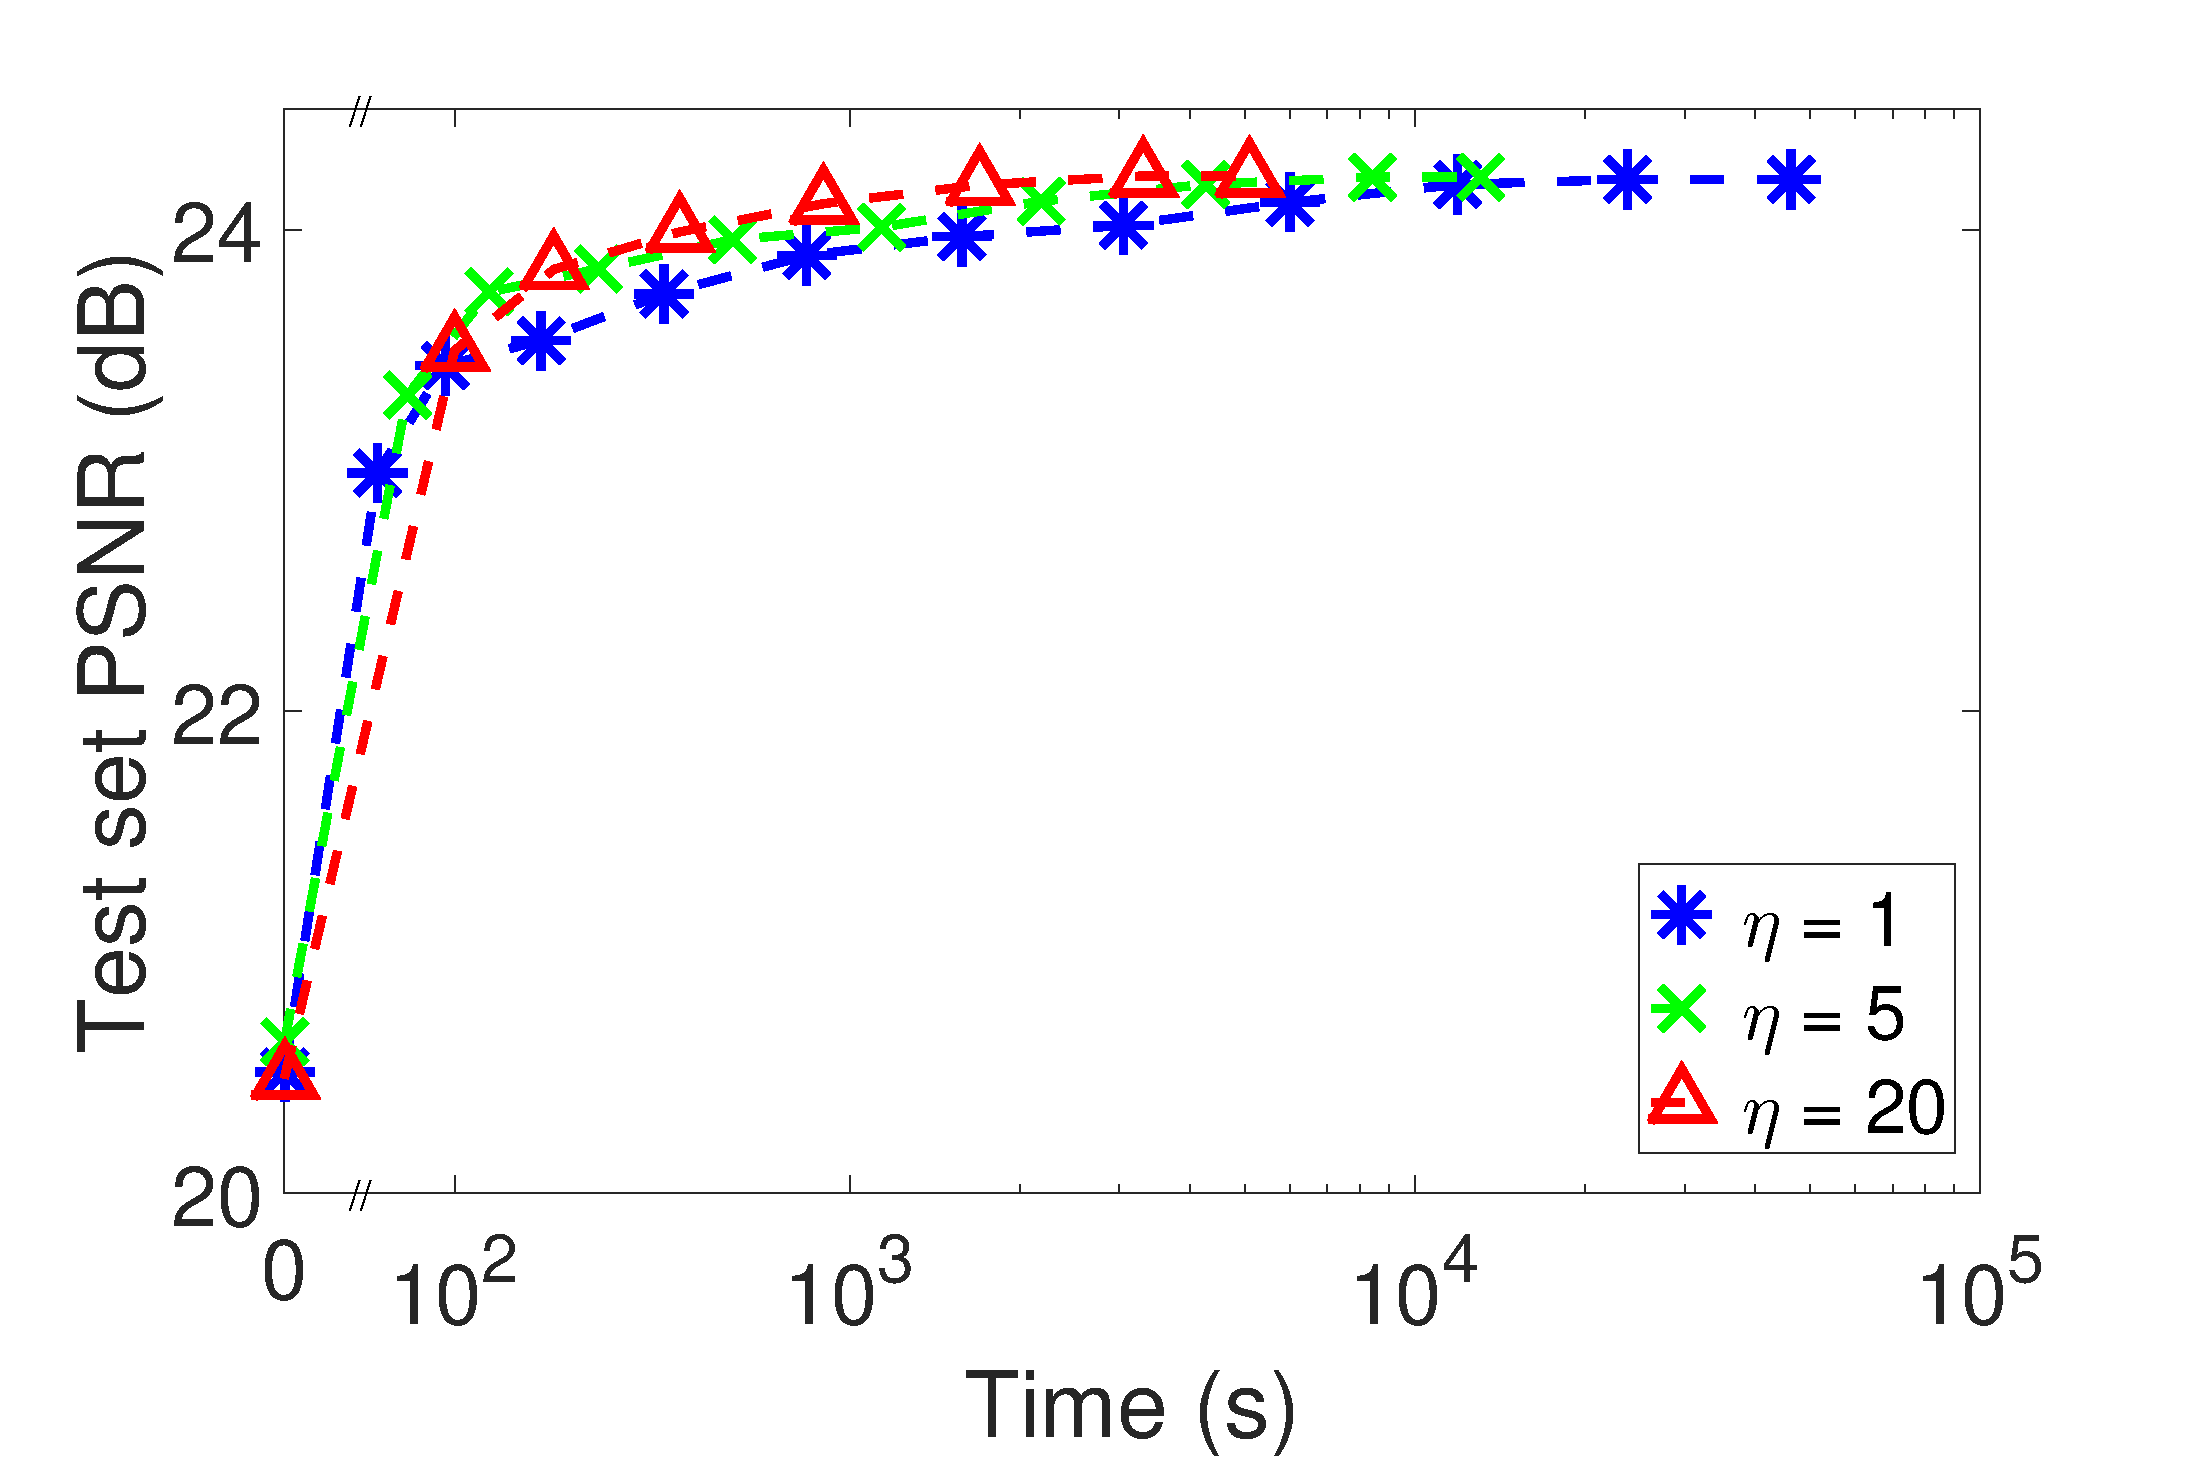
\includegraphics[width=1\linewidth]{figure/minibatch.pdf}
\end{subfigure}

\caption{Top: Testing PSNR for the comparable method~\cite{liu-2018-first} with $K=100$, and our method (SOCSC) with $K=100$ and $K=400$, respectively. Every iteration draws a single image from those 1000 image patches. Bottom: Testing PSNR for SOCSC ($K=400$) with varying values of $\eta$. The learned filters are examined on the test sets every $2^i$ iterations and also at the last iteration, where $i=0,1,\dots$. Note that all the results are generated by a single-core program.}
\label{fig:overComDicAndMinibatch}
\end{figure}

The runtime comparisons for various mini-batch sizes are shown in the
bottom of Fig.~\ref{fig:overComDicAndMinibatch}. Note that larger
$\eta$ will result in a smaller number of iterations to process all
$1000$ samples. The plots show that a larger mini-batch size will
generally lead to a greater progress in first few training steps,
though it takes additional running time and memory. Overall,
mini-batched update provides a more runtime efficient learning
process in the online-based CSC model, and according to the obtained
experimental results, $\eta=20$ achieves one order of magnitude
speedup over $\eta=1$ to reach a a comparable level of
convergence. Since computing sparse codes is a data-independent
process, this mini-batched approach can be further accelerated in a
distributed-computing system.



% --- DO NOT DELETE ---
% Local Variables:
% mode: latex
% mode: flyspell
% mode: TeX-PDF
% End:

